\chapter{Empirical Evaluation}
\label{chapter:evaluation}

\par In this chapter, we report and discuss a comprehensive set of experiments to evaluate the performance of our pattern prediction system. We make use of both synthetic and real-word event streams. Section~\ref{sec:exp_setu} provides a brief overview of the used event streams for our evaluation and the experimental environment. Section~\ref{sec:metrics} introduces the metrics used for the evaluation. In Section~\ref{sec:results_real} and ~\ref{sec:results_synthetic}, the evaluation results of our system over synthetic and real-world event streams are reported. Finally, Section~\ref{sec:throughput} discusses the scalability evaluation of the proposed system.  

%In next, we present the experimental setup, and discuss the results of the proposed method.   
%Effects of parameters
\section{Setup}
\label{sec:setup_data}

\subsection*{Experimental setup}
\label{sec:exp_setu}
\par We ran our experiments on a single-node standalone Flink cluster deployed on an Ubuntu Server 17.04 with Intel(R) Core(TM) i7-7700 CPU @ 3.60GHz X 8 processors and 32GB RAM. We used Apache Flink v1.4.0 and Apache Kafka v0.10.2.1 for our experiment.

\par We also conducted experiments to measure the throughput of our system on a YARN \cite{vavilapalli2013apache} cluster (v2.7.2) with 9 physical nodes, where each node has 10 cores CPU, and 100 GB memory. More information about the deployment on the YARN cluster can be found on the source code repository \footnote{ \url{https://github.com/ehabqadah/distributed_online_learning_for_large-scale_pattern_prediction}}.



\subsection*{Experimental Streams}

\subsubsection*{Real-word Event Streams}
We used real-world event streams provided by the datAcron project in the context of maritime monitoring. These event streams describe critical points (i.e., synopses) of moving vessels trajectories, which are derived from raw AIS messages as described in \cite{synopses1}. In particular, for our evaluation experiments we used a data set of synopses that contains $4,684,444$ critical points of $5055$ vessels that sailed in the Atlantic Ocean during the period from 1 October 2015 to 31 March 2016.

\par We used the synopses data set to generate a simulated stream of event tuples  i.e., \textit{(id, timestamp, longitude, latitude, annotation, speed, heading)}. The  system further processes the stream to attach an extra event \textit{type} attribute,  where $type$ $\in \Sigma1$ or $type$ $\in \Sigma2$.


\par $\Sigma_1=$$\{$\textit{VerySlow, Slow, Moving,  Sailing, Stopping}$\}$, which is based on a discretization of the speed values. That is, $\Sigma_1$ includes a simple derived event types based on the speed value that can be used over streams of  raw AIS  or critical points. While $\Sigma_2=$ $\{$\textit{stopStart, stopEnd, changeInSpeedStart, changeInSpeedEnd,  slowMotionStart, slowMotionEnd, gapStart, gapEnd, changeInHeading}$\}$, which is derived based on the values of the $annotation$ attribute that encodes the extracted trajectory movement events \cite{synopses1}. $\Sigma_2$ represents the set of possible mobility changes in the vessel's trajectory \cite{synopses1}, each critical point has at least one event. Where in the case of multiple values we generate duplicate points each of which corresponding to one event in the same order of $\Sigma_2$.

\par In our experiments, we monitor a pattern $\mathcal{P}_1=Sailing$ with $\Sigma_1$ that detects when the vessel is underway (sailing). Likewise, we test a second pattern  $\mathcal{P}_2=$\textit{changeInHeading; gapStart; gapEnd; changeInHeading} with $\Sigma_2$ that describes a potential illegal fishing activity \cite{alevizos2017event}. 


\subsubsection*{Synthetic Event Streams}

\par In order to get a better insight of our proposed approach, we evaluate it on synthetic event streams. For our experiments, we generate $20$ streams of size 10,000 events from a simulated 1-order Markov process over $\Sigma=\{a, b, c, d\}$.

\par We define a simple pattern $\mathcal{P}=a ; d ; c$ to study the predictive performance along with the learning efficiency of the transition probability matrix of the Markov chain source.  We compare the learned matrix of \pmcmr models in our approach and the isolated case to the used transition matrix to generate the streams. We map the transition probability matrix of the \pmcmr and the transition probability matrix of the Markov chain source as was mentioned earlier in Section ~\ref{sec:underlaying_mc}.
   


\section{Evaluation Metrics} 
\label{sec:metrics}
\par We compare our proposed system, which enables the synchronization of prediction models (i.e., \pmcmr models) on the distributed predictor nodes,  against the isolated prediction mode, in which models are computed on single streams only. We compare the performance in terms of following metrics:
\begin{itemize}	
	\item  $\mathit{Precision} =$ $ \mathit{\frac{\#\ of\ correct\ predictions}{\#\ of\ total\ predictions}}$. The fraction of the predictions that are correct. For each new event in the stream, the predictor provides a prediction interval where the full match of the pattern might occur. Thus, the predictions are temporarily stored until a full match is detected. At that point, all stored prediction intervals are evaluated by considering those intervals where the full match occurred within as correct.     
	\item $\mathit{Spread}\ $=$\ end(I) -start(I)$. The width of the prediction interval $I$, which represents the number of events between the start and the end of $I$.
	\item $\mathit{Distance}\ $=$\ start(I) - now$. The distance between the start of the prediction interval $I$ and the time of prediction is produced (now). The  higher distance represents the earlier prediction of the pattern full match \cite{alevizos2017event}.  
		
	\item $\mathit{PS-}$score = $\alpha * precision + (1 - \alpha ) * ( 1- \frac{spread}{max\  spread})$. In analogy with the $F-score$ we introduce this new score to assess the performance of the system in terms of both the $\mathit{precision}$ and the $\mathit{spread}$ combined.
	\item  $\mathit{Cumulative\ communication}$. We study the communication cost by measuring the $\mathit{cumulative\ communication}$ that captures the number of messages, which are required to perform the distributed online learning modes to synchronize the prediction models.	
\item $Throughput$. The number of events processed per unit time (second).
\end{itemize} 

Our proposed system can operate in three different modes of synchronization schemes: 
\begin{enumerate}[label=(\roman*)] 
	\item continuous full synchronization for each incoming event (hypothetical).
	\item static scheme based on synchronizing the prediction models periodically every $b$ of input events in each stream.
	\item dynamic synchronization protocol based on making the predictors communicate their local prediction models periodically but only under condition that the divergence of the local models from a reference model exceeds a variance threshold $\Delta$ (recommended).  	   
	
\end{enumerate}

In our experiments, we compare the distributed online learning modes against the the setting where the \pmcmr predictors work in isolation. 

\section{Results on Real-word Event Streams}
\label{sec:results_real}

In this section, we present the experimental results for two different patterns  $\mathcal{P}_1=Sailing$ (with an order of )$m=2$), and   $\mathcal{P}_2=$\textit{changeInHeading; gapStart; gapEnd; changeInHeading} (with first order $m=1$). All experiments are performed with the batch size of 100  ($b=100$), the variance threshold of 2 ($\Delta=2$), $80\%$ as PMC prediction threshold ($\theta_{p}=80\%$), and 200 for the maximum spread ($\theta_{s}=200$).

\begin{figure}[H]
	\centering
	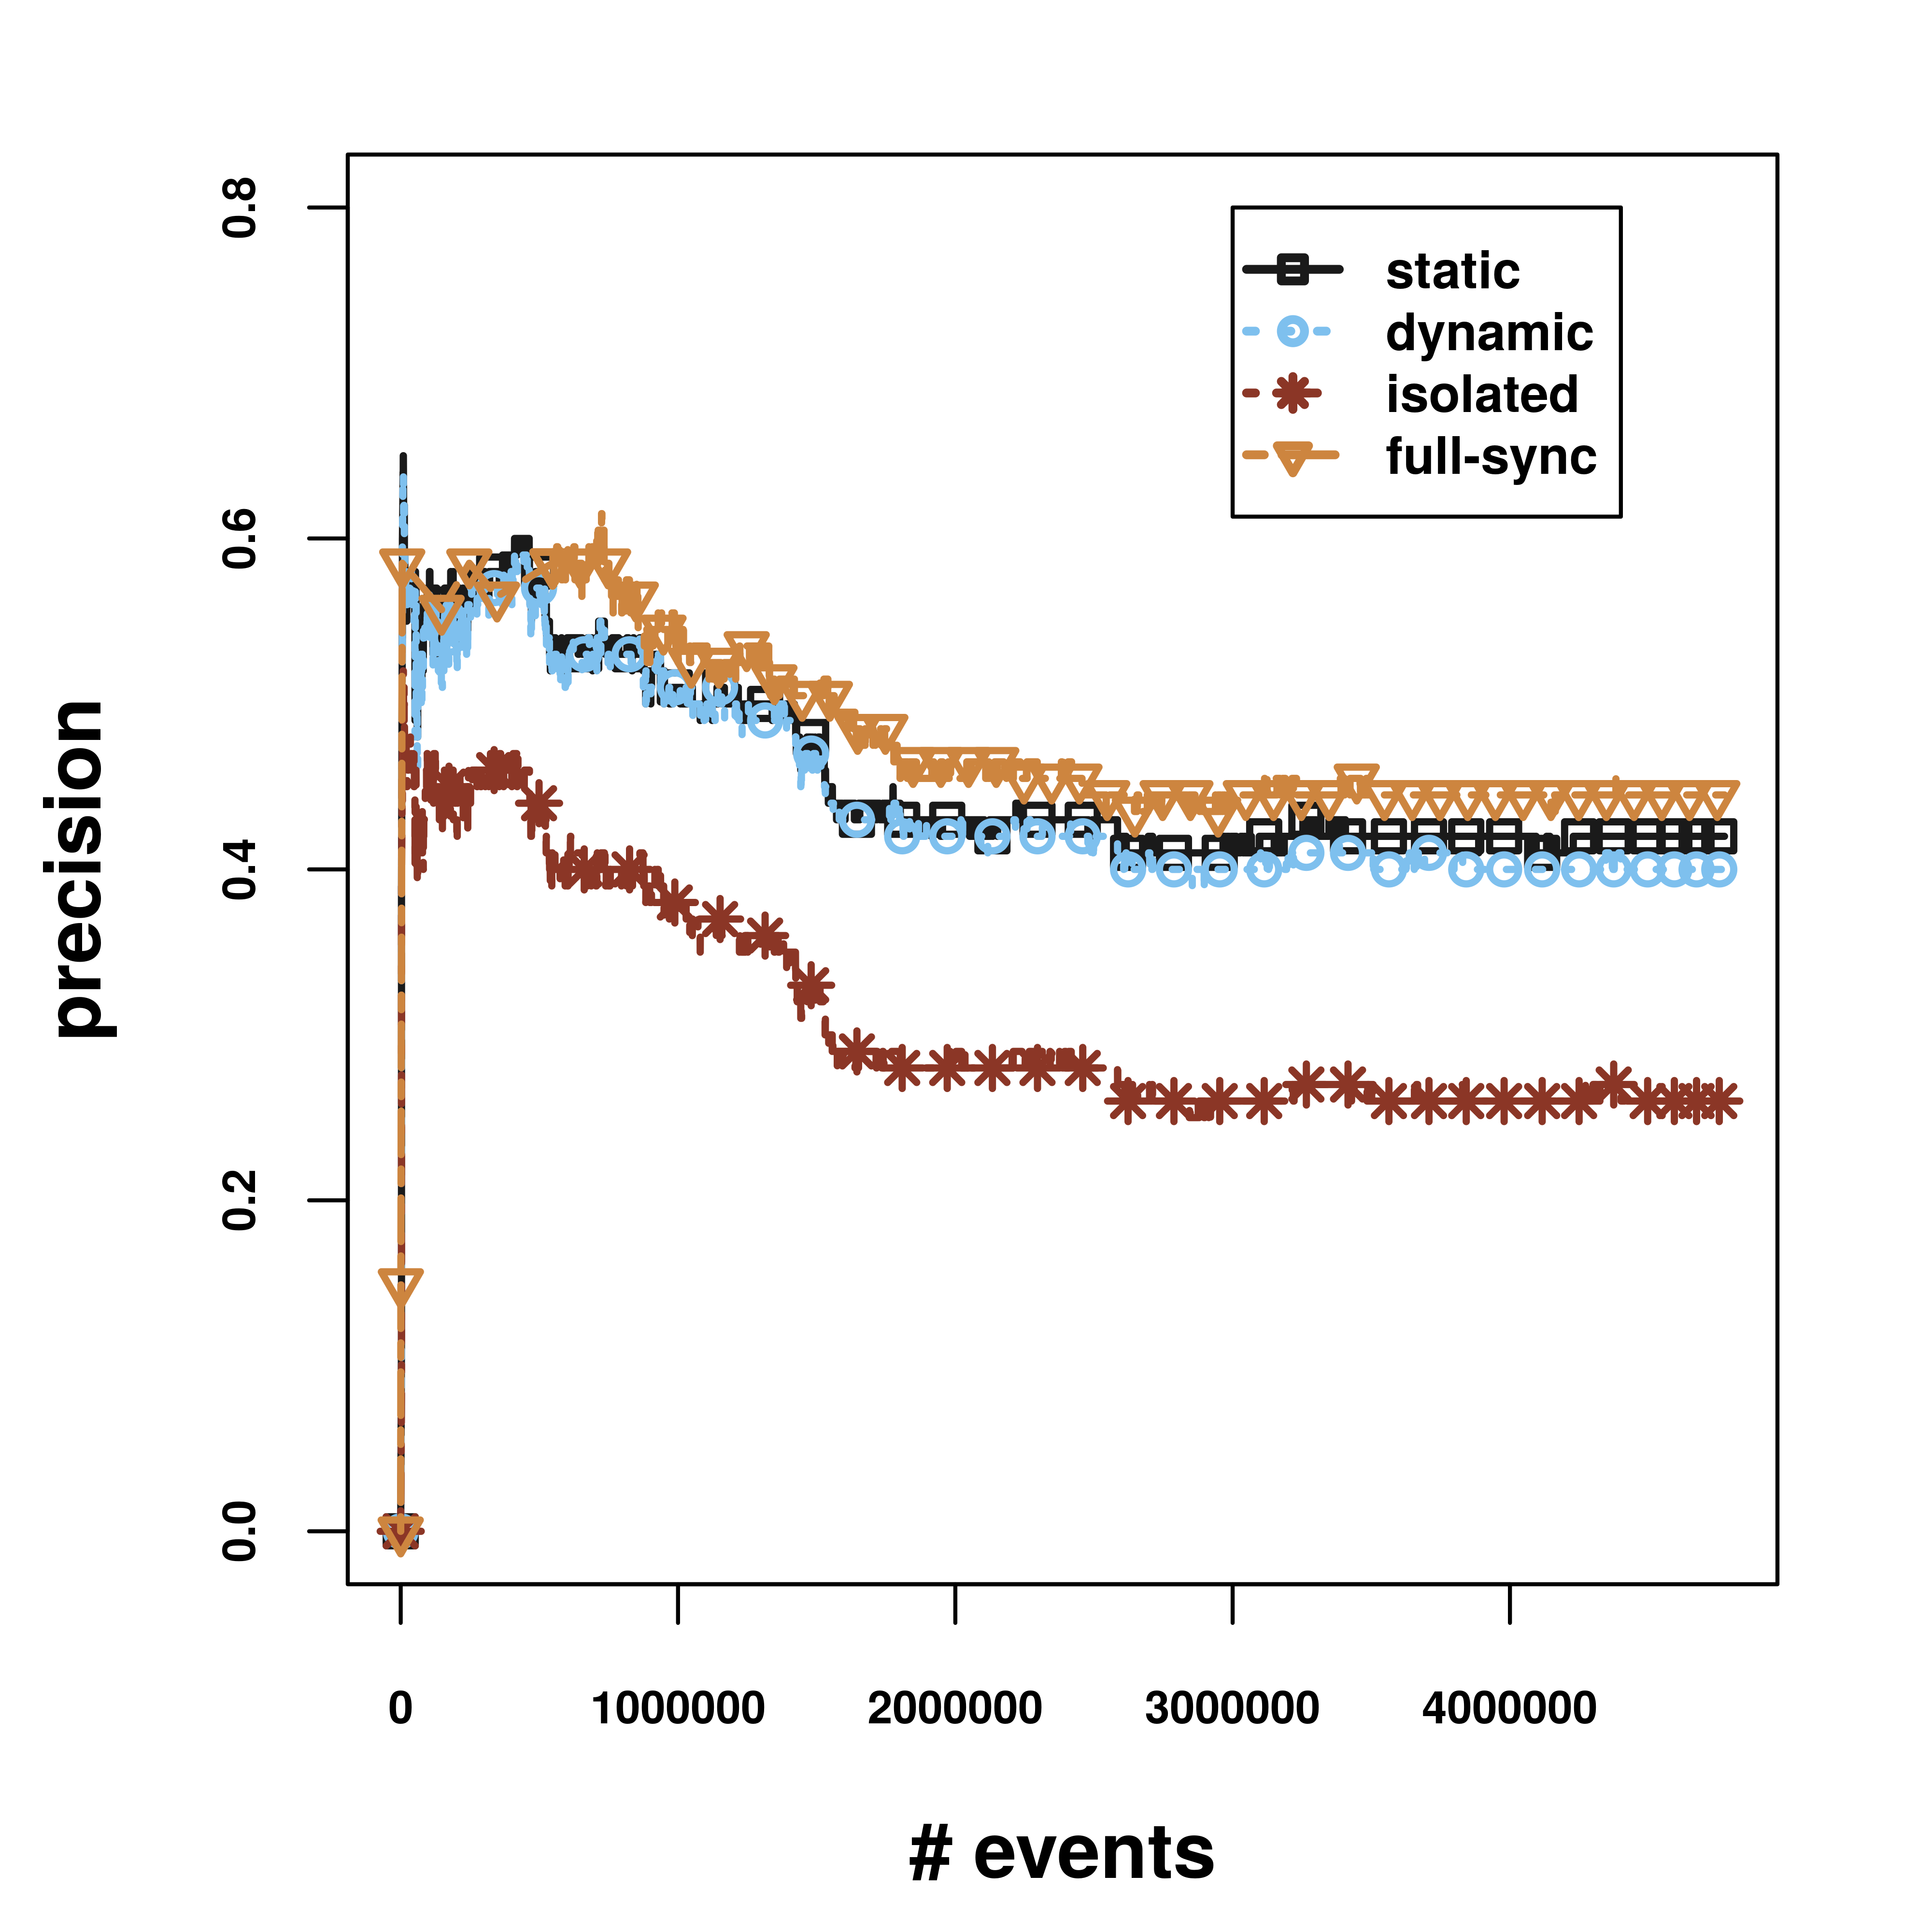
\includegraphics[width=\textwidth,keepaspectratio]{chapters/figures/synopses/new/precision_p1.png}
	
	\caption{Precision scores with respect to the number of input events over time for $\mathcal{P}_1$.}
	\label{fig:precsions}
\end{figure}

\par Figure~\ref{fig:precsions} depicts the average precision scores of predictions models for the first pattern $\mathcal{P}_1=Sailing$ (one prediction model per vessel) of all synchronization modes, namely, isolated without synchronization, continuous (full-sync), static, and our recommended approach based on the dynamic synchronization scheme. It can be clearly seen that all methods of distributed learning outperform the isolated method. The full continuous synchronization method has the highest precision rates, while the static and dynamic synchronization schemes have close precision scores. Consequently, dynamic synchronization is not much weaker than the static synchronization, but requires much less communication, as explained below.


\begin{center}
	
	\begin{figure}[H]
		\centering
		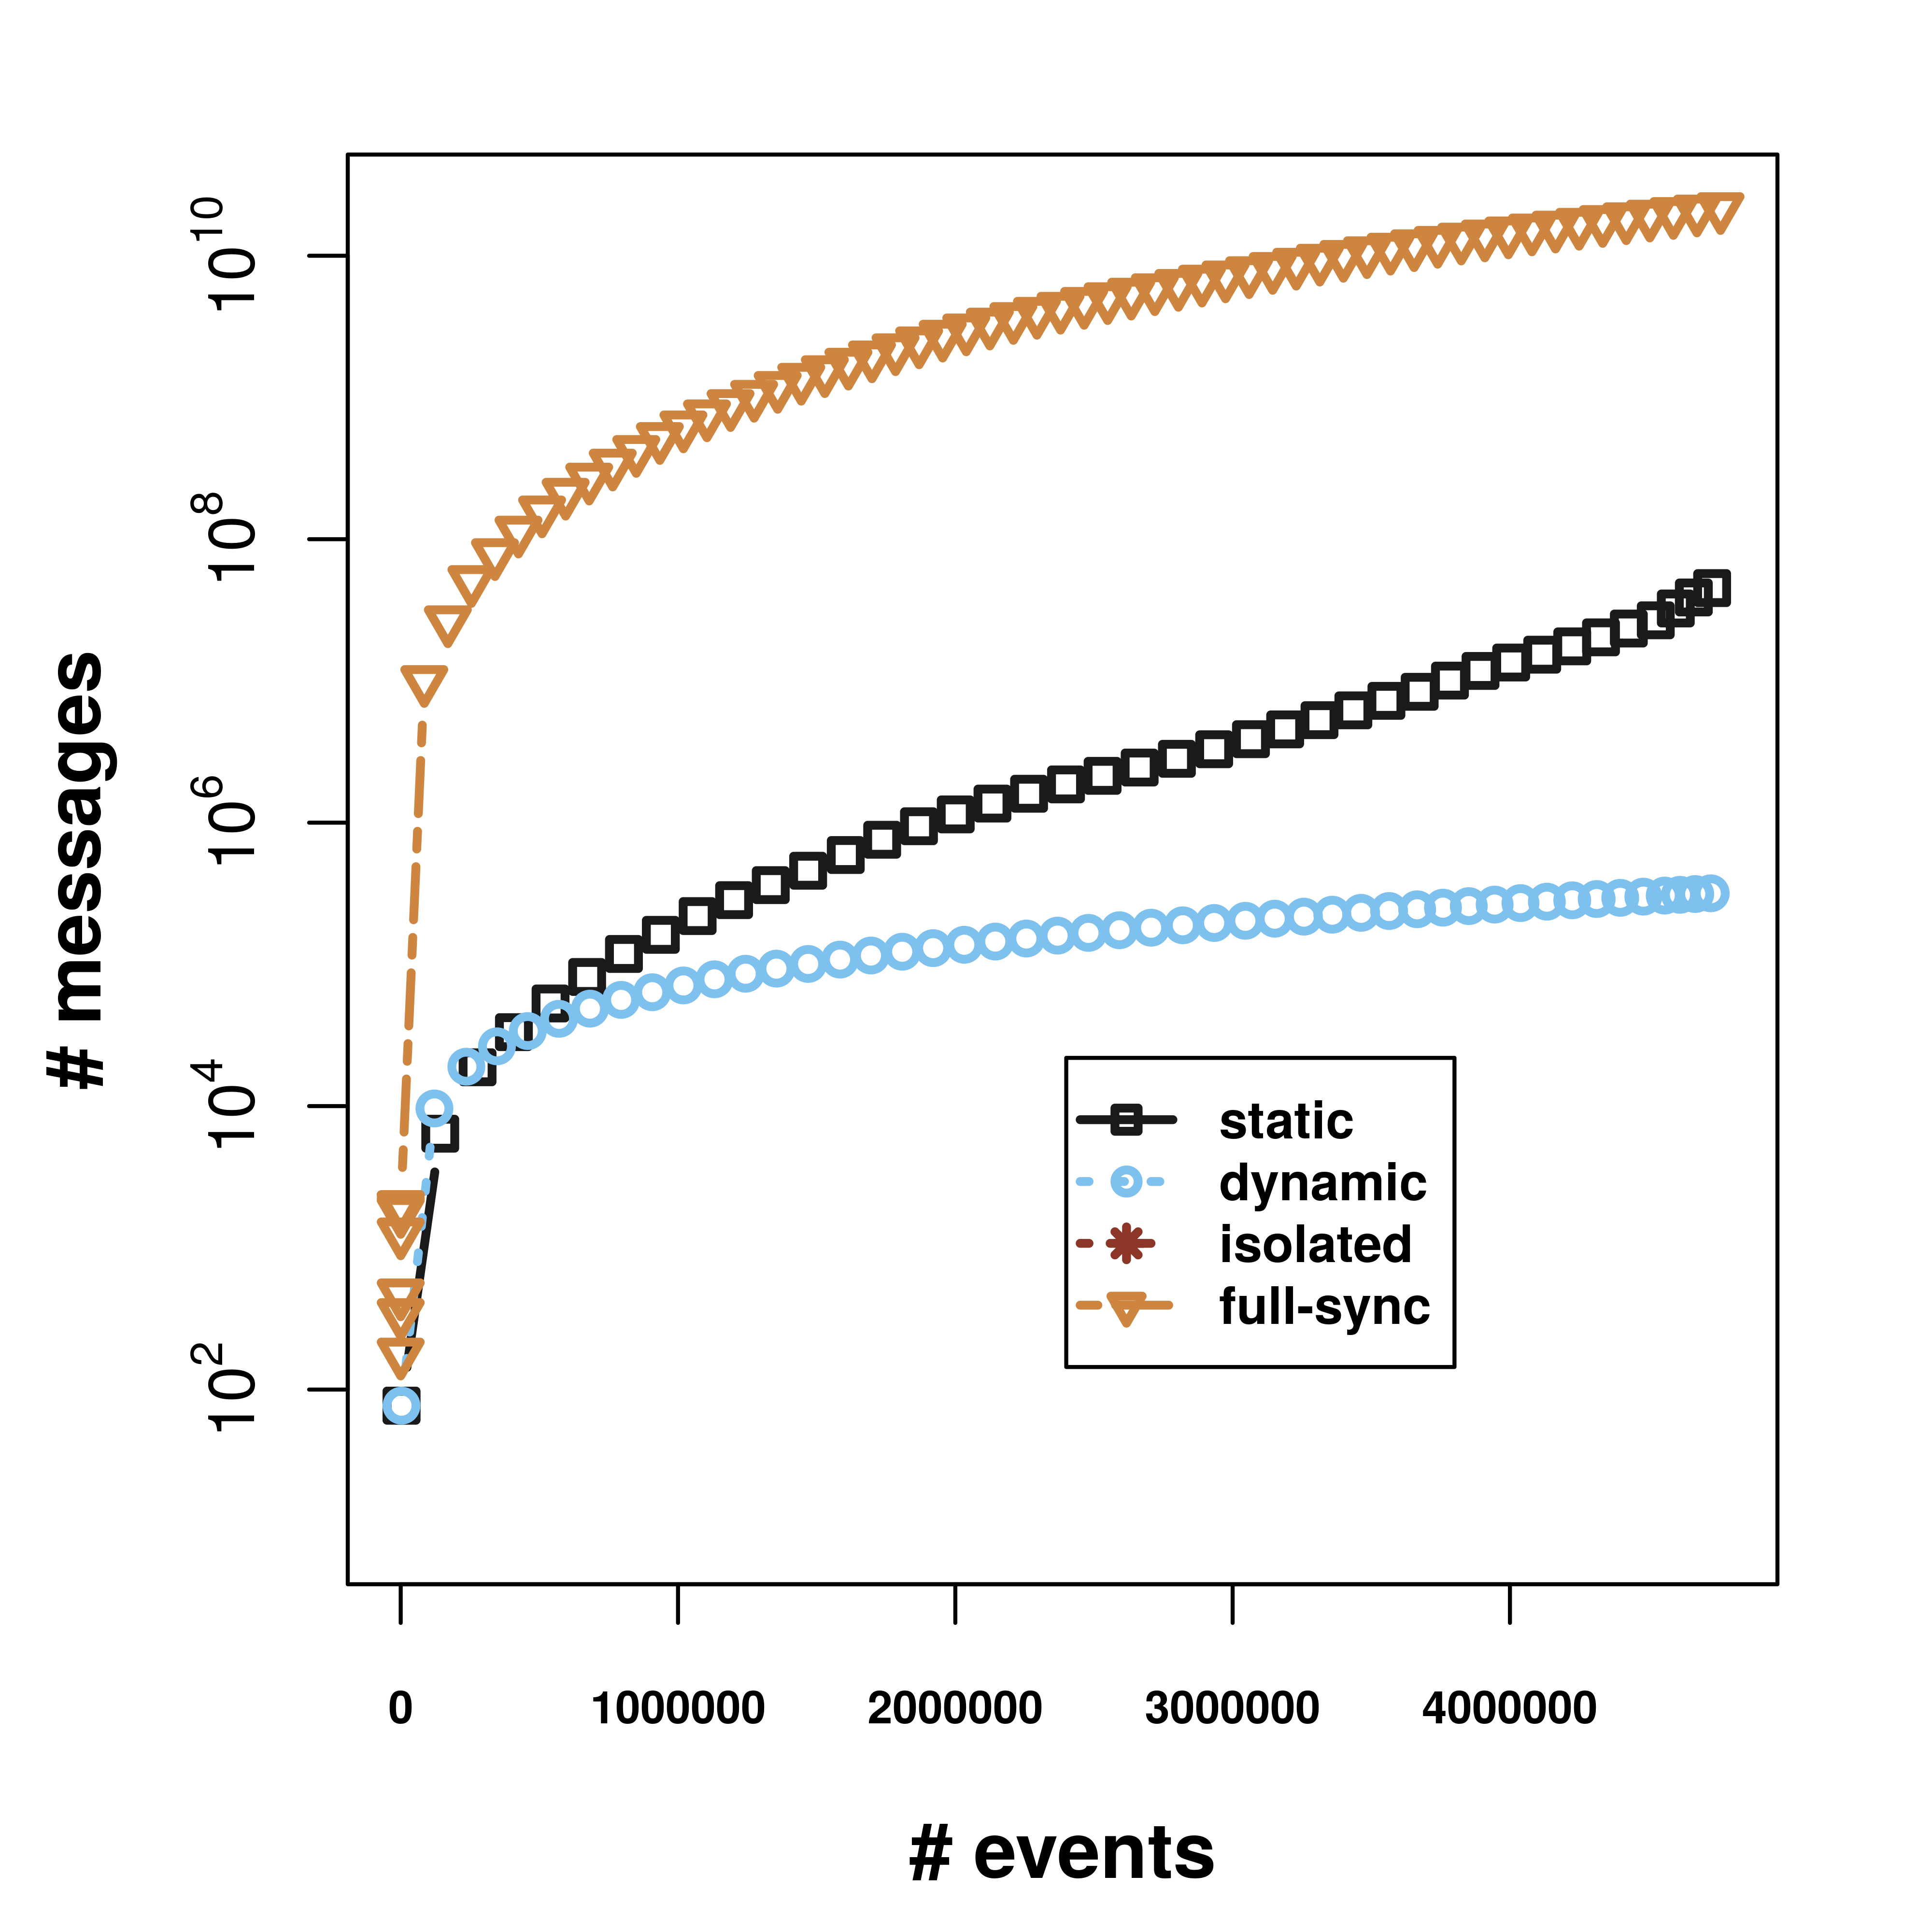
\includegraphics[width=\textwidth,height=.9\textwidth,keepaspectratio]{chapters/figures/synopses/new/messages_p1.png}
		
		\caption{Cumulative communication with respect to the number of input events over time for $\mathcal{P}_1$.}
		\label{fig:comm}
	\end{figure}
\end{center}

\par Figure~\ref{fig:comm} provides the accumulated communication cost that is required by the three distributed online learning modes, while the isolated approach does not require any communication at all. These results are shown for $\mathcal{P}_1$.  As expected, a larger amount of communication is required for the full synchronization comparing to the static and dynamic approaches. Also, it can be seen that we can reduce the communication overhead by applying the dynamic synchronization protocol (a reduction by a factor of 100) compared to the static synchronization scheme, even with a small variance threshold $\Delta=2$. Furthermore, the dynamic  protocol still preserves a similar predictive performance to the static one as illustrated in Figure~\ref{fig:precsions}.  Therefore, we will only consider the dynamic synchronization and the isolated approach in the evaluation of the second pattern.


%As counterintuitive as it may seem, population sizes don’t go up as the world gets healthier. They go down. Here’s why.

\begin{center}
	
	\begin{figure}[H]
		\centering
		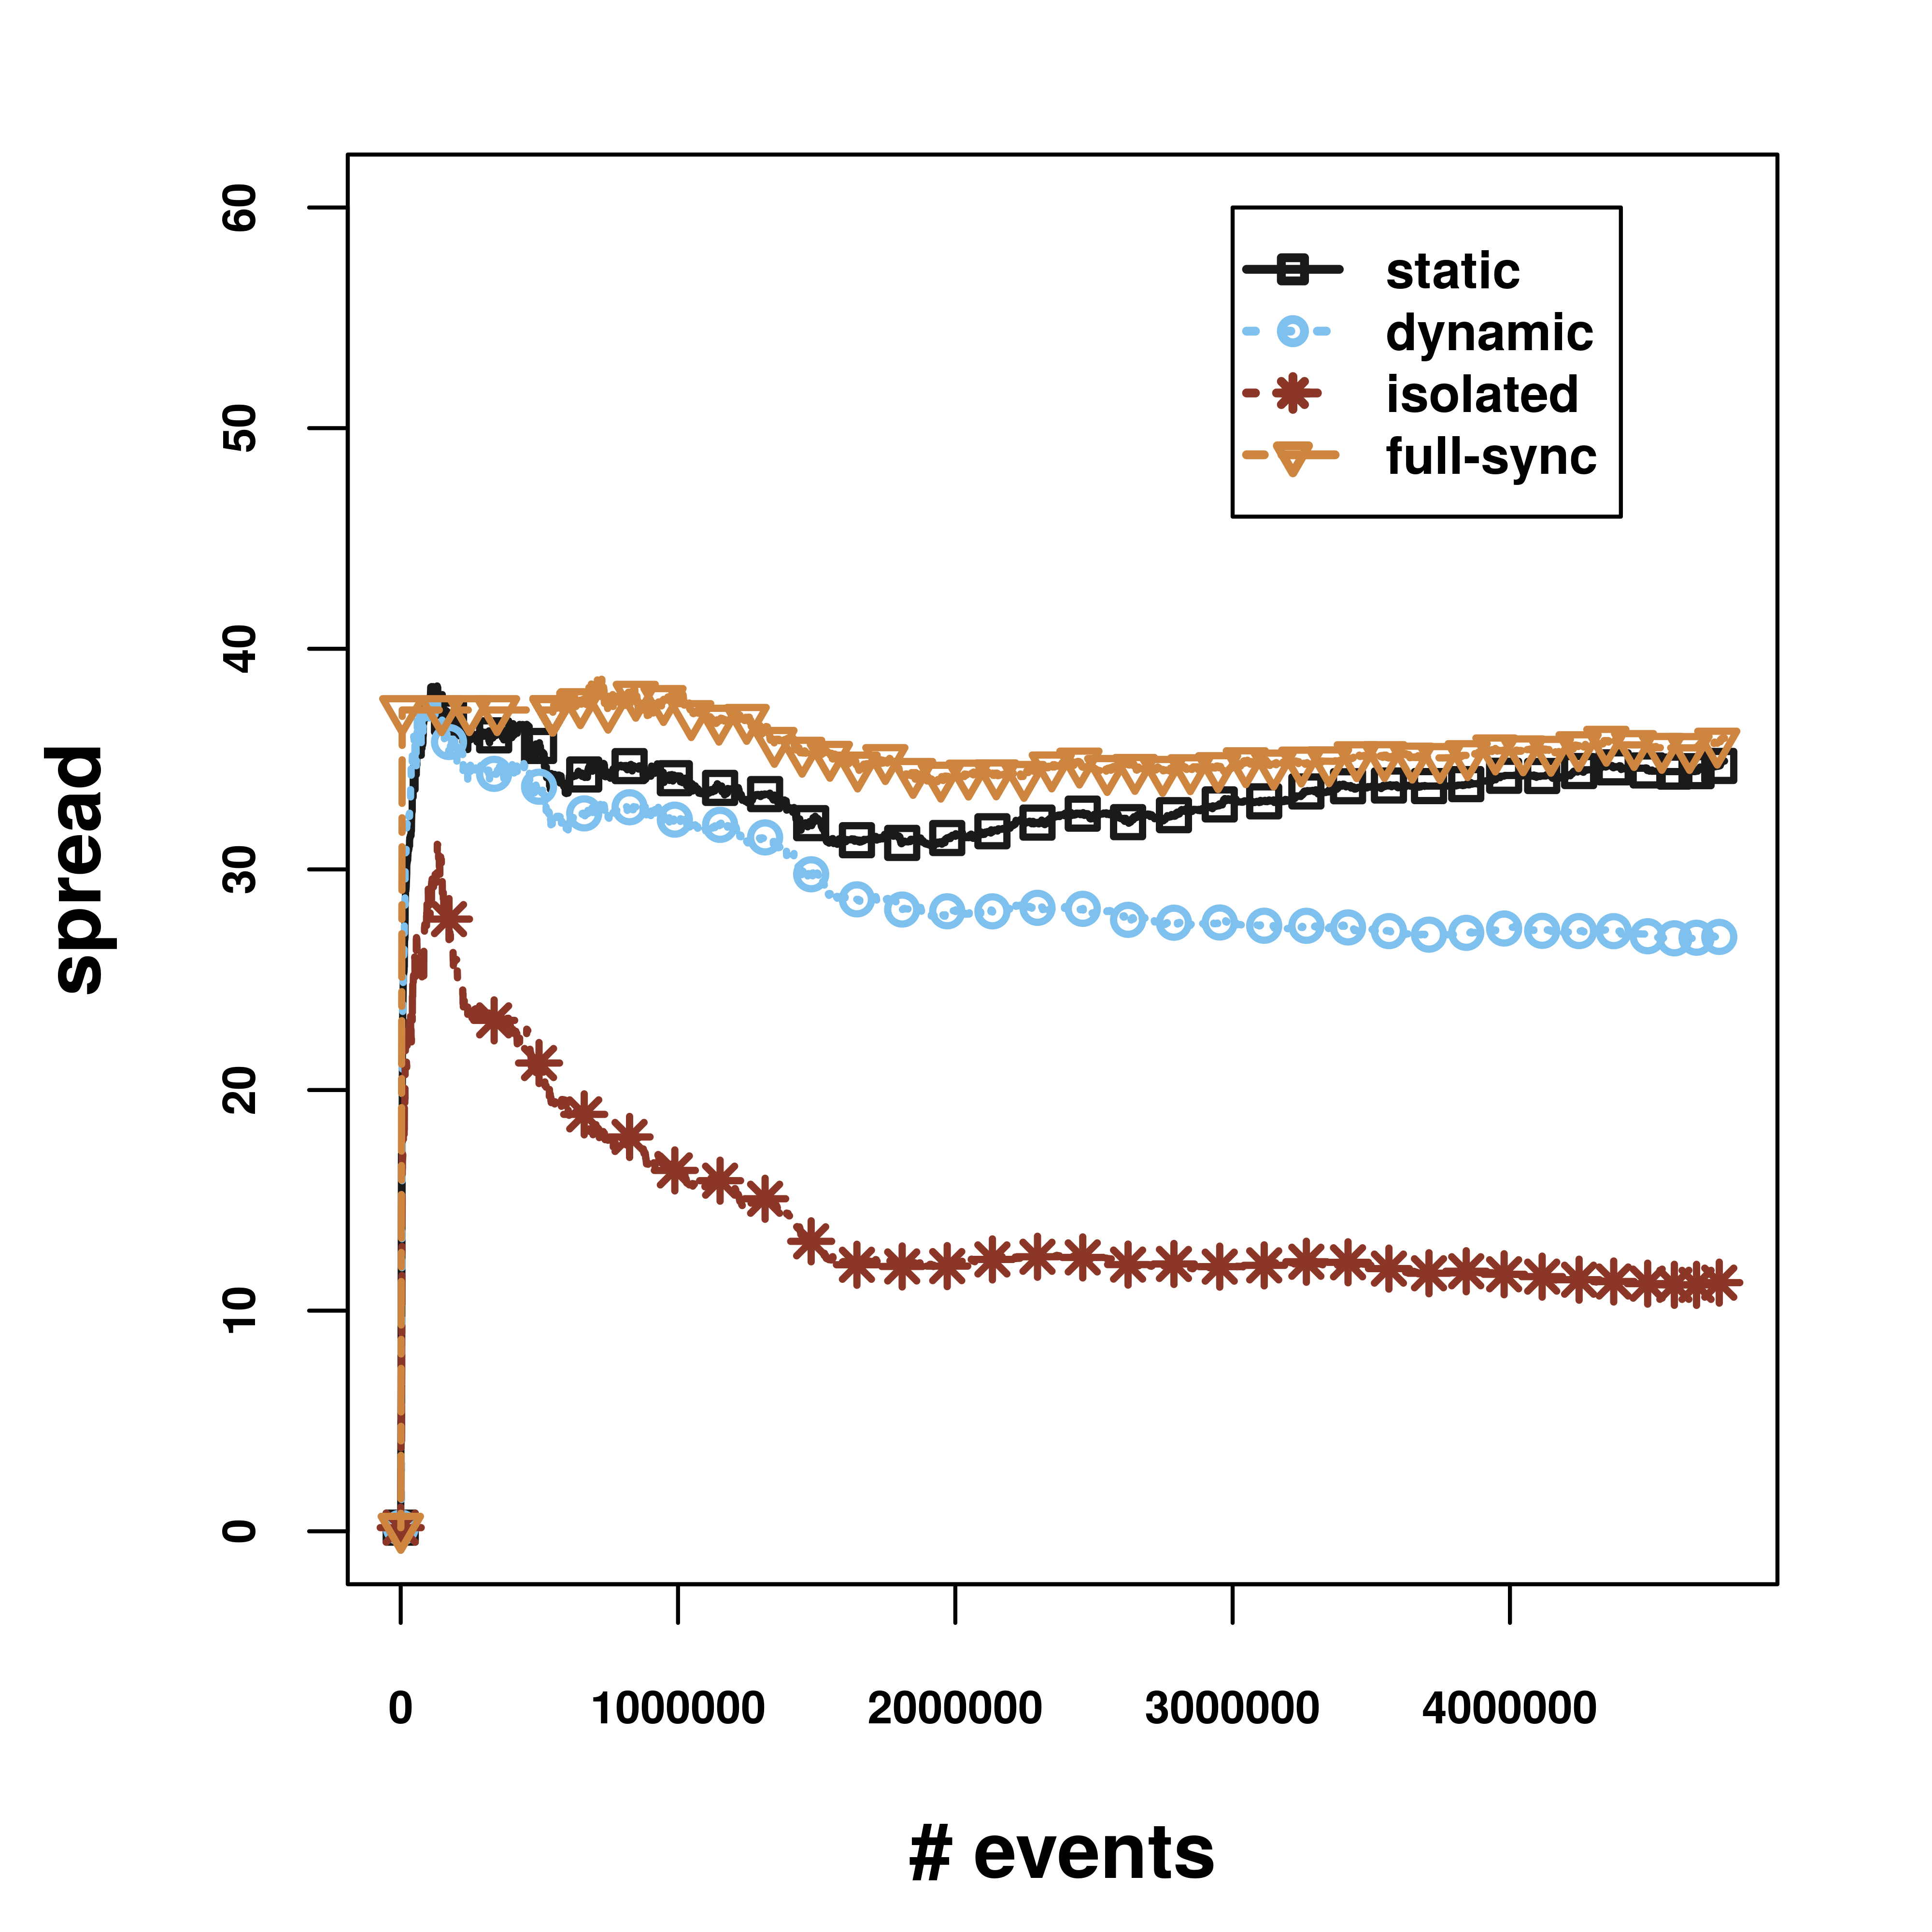
\includegraphics[width=\textwidth,height=.9\textwidth,keepaspectratio]{chapters/figures/synopses/new/spread_p1.png}
		
		\caption{Average spread for $\mathcal{P}_1$.}
		\label{fig:spread}
	\end{figure}
\end{center}

\par In Figure ~\ref{fig:precsions}, we observe that the precision decreases initially and then stabilizes. This seems to be counter-intuitive, as we expect the models to improve up to a certain point as it get more data. We  investigated the effect of the distributed synchronization of the prediction models on the average spread value, Figure  ~\ref{fig:spread}  shows the spread results for all approaches. It can be seen that the spread is higher for the distributed learning based methods comparing to the isolated approach. Furthermore, the average spread decreases over time until convergence, as result of confidence increase in the models, which is inherited from the \pmcmr models. 

\par For a clearer picture of the comparison between our distributed learning method and the isolated approach, Figure ~\ref{fig:spread_prec} depicts the $PS$-score for $\mathcal{P}_1$. It is clear that our approach achieves better performance in terms of the precision and spread combined.  

\begin{center}
	\centering
	\begin{figure}[H]
		
		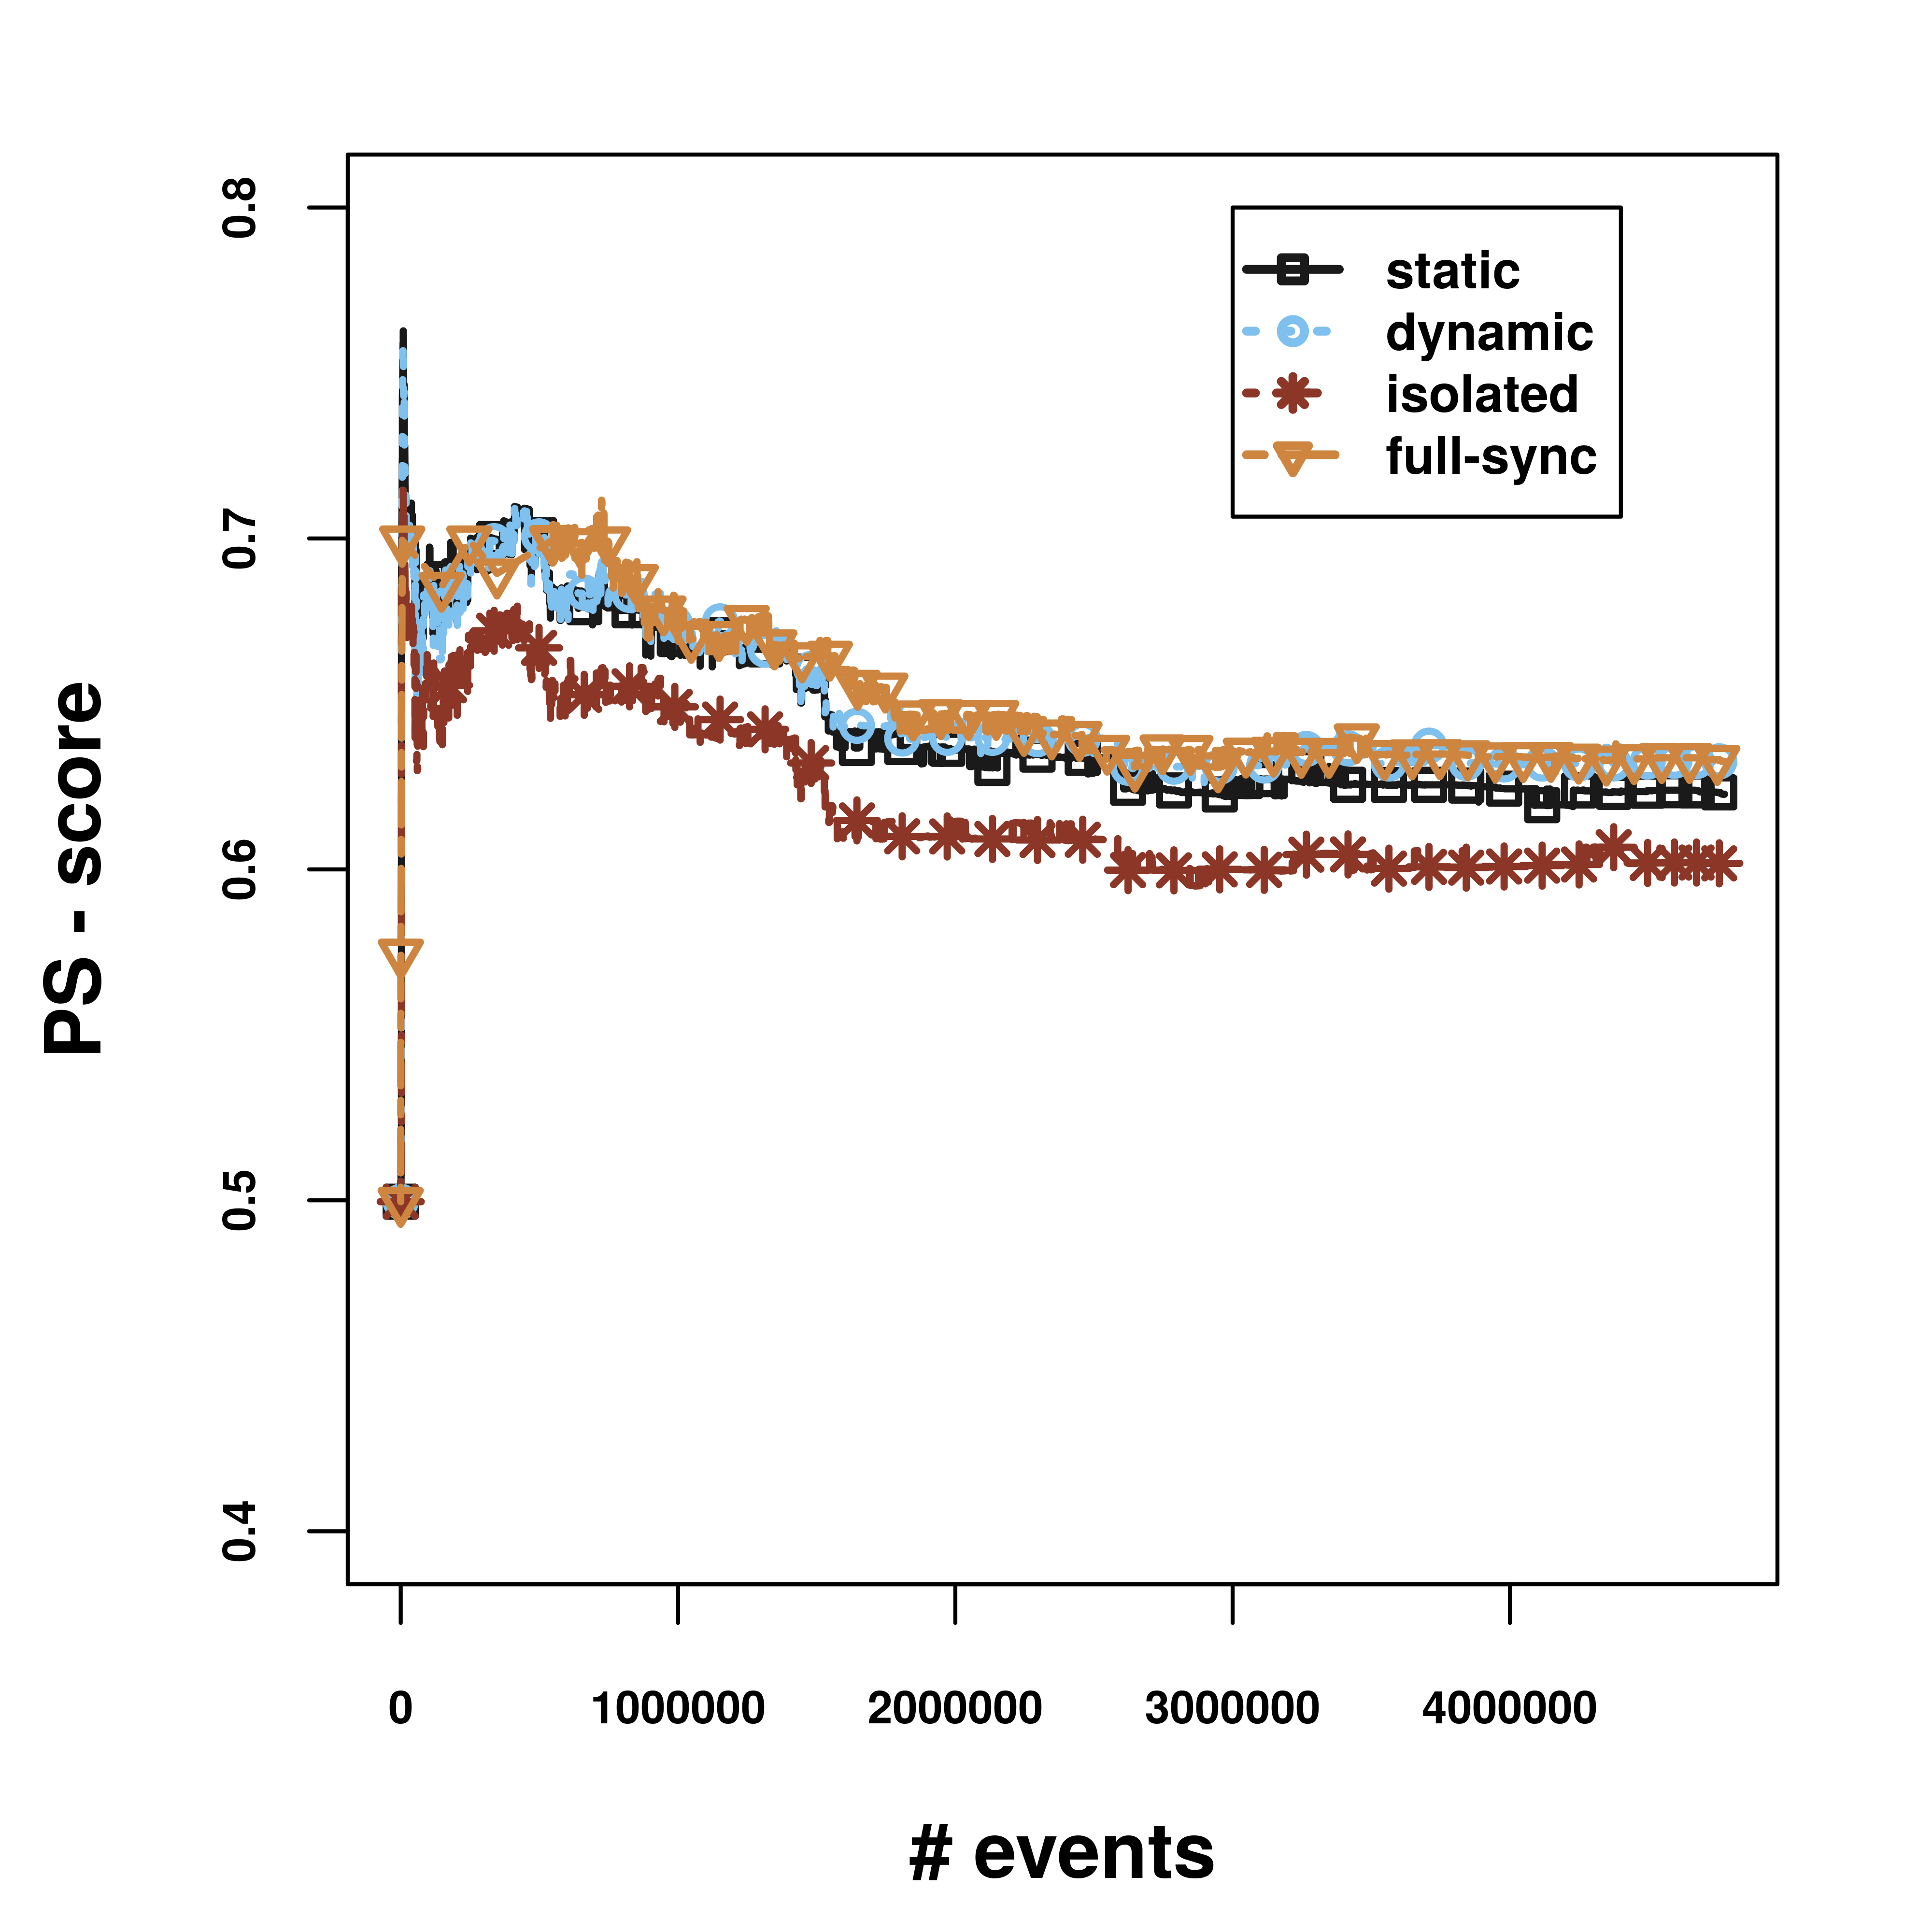
\includegraphics[width=\textwidth,height=.9\textwidth,keepaspectratio]{chapters/figures/synopses/new/ps_score_p1.png}
		
		\caption{$PS$-score for $\mathcal{P}_1$ with $\alpha = .5$.}
		\label{fig:spread_prec}
	\end{figure}
\end{center}



\begin{center}
	\centering
	\begin{figure}[H]
		
		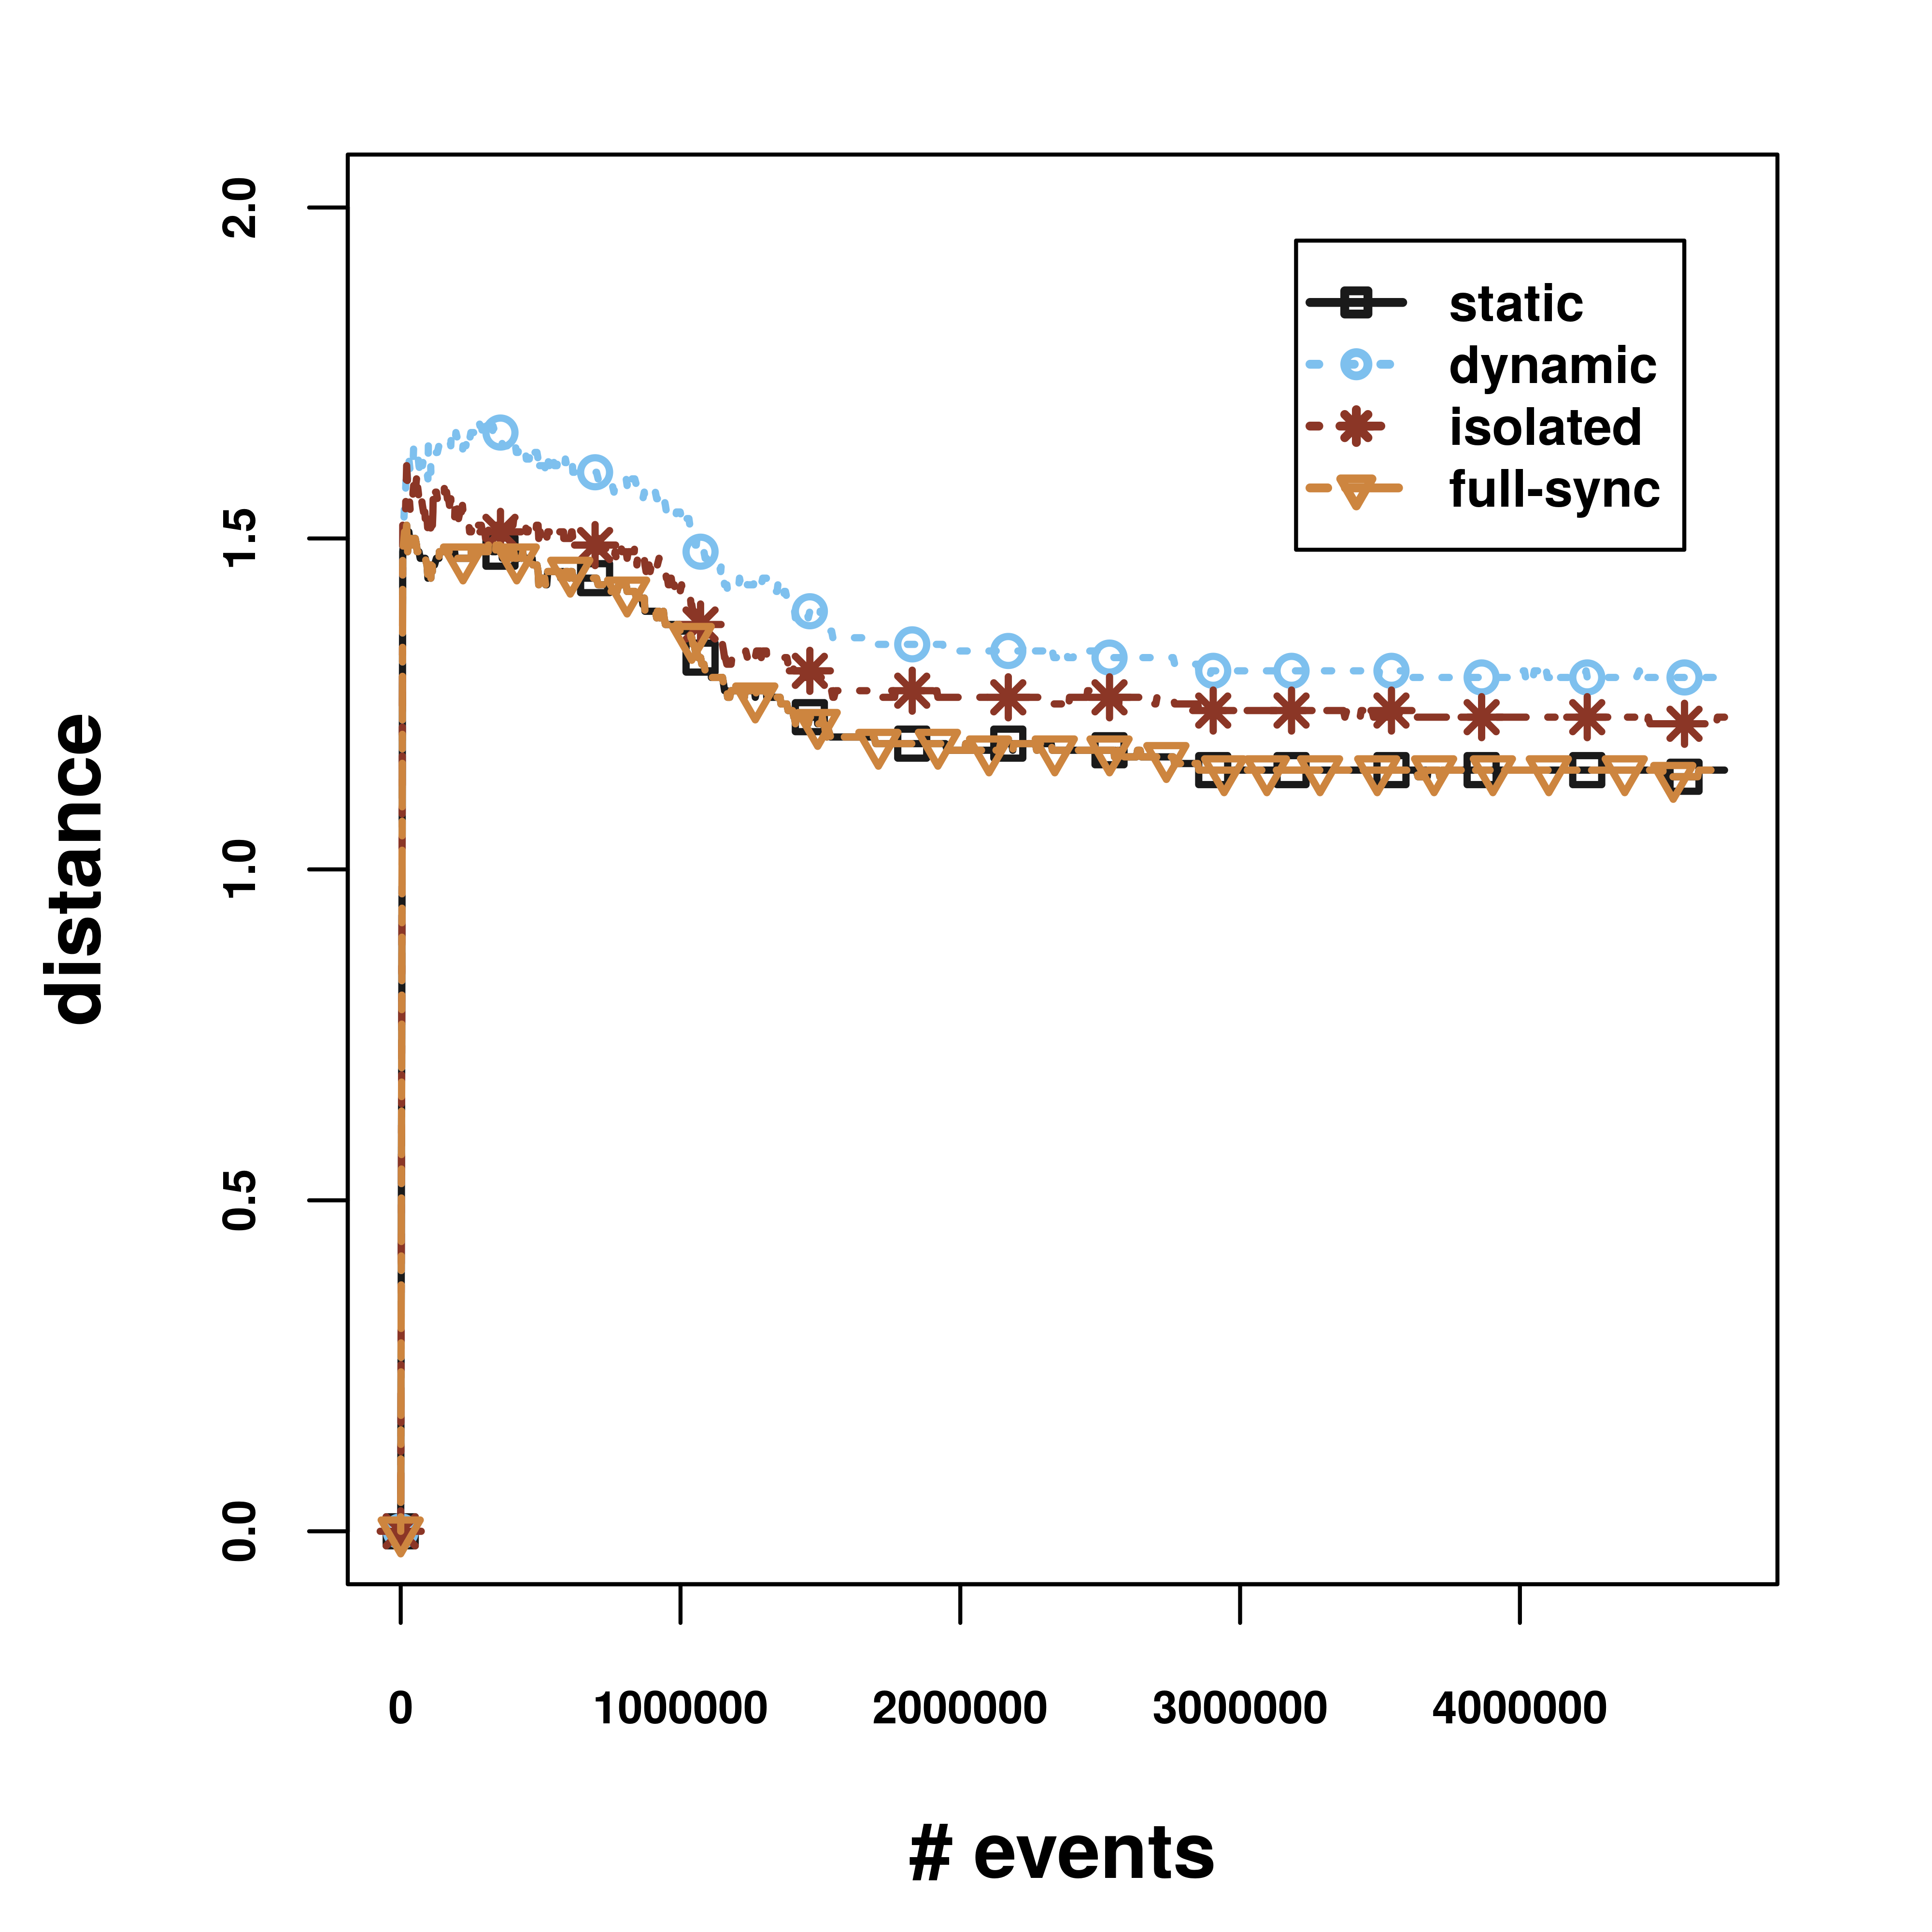
\includegraphics[width=\textwidth,height=.9\textwidth,keepaspectratio]{chapters/figures/synopses/new/distance_p1.png}
		
		\caption{Distance for $\mathcal{P}_1$.}
		\label{fig:distance_p1}
	\end{figure}
\end{center}

On the other hand, Figure~\ref{fig:distance_p1} reports the average of the distance metric for all approaches. As can be seen, the dynamic synchronization method has the higher distance values (i.e., earlier predictions of the full matches). It can also be seen that the isolated has a slightly better distance.  


\par For the second, more complex pattern ($\mathcal{P}_2$), we have found that the precision was worse for a distributed model generated over all vessels than in the model created for each vessel in isolation. This indicates that there is no global model describing the behavior of all models consistently. However, when we look at specific groups of vessels, we achieve an improvement in terms of precision. As initial experiment, we only enable the synchronization of the prediction models associated with vessels that belong to the same vessel class. Currently, this change is technically performed by an extra filter step that passes only one type of vessels, while multiple runs of the system are required for all vessel types. For example, Figure ~\ref{fig:precsions_p2} shows the precision scores for vessels of class \textit{pleasure craft}. This case might seem to contradict of our assumption that the input event streams belong to the same distribution and share the same behavior, but it actually follows the same assumption but between the predictors of vessels within the same type group. An interesting observation is that the dynamic synchronization approach still has a higher precision scores than the isolated approach.

\begin{figure}[H]
	\centering
	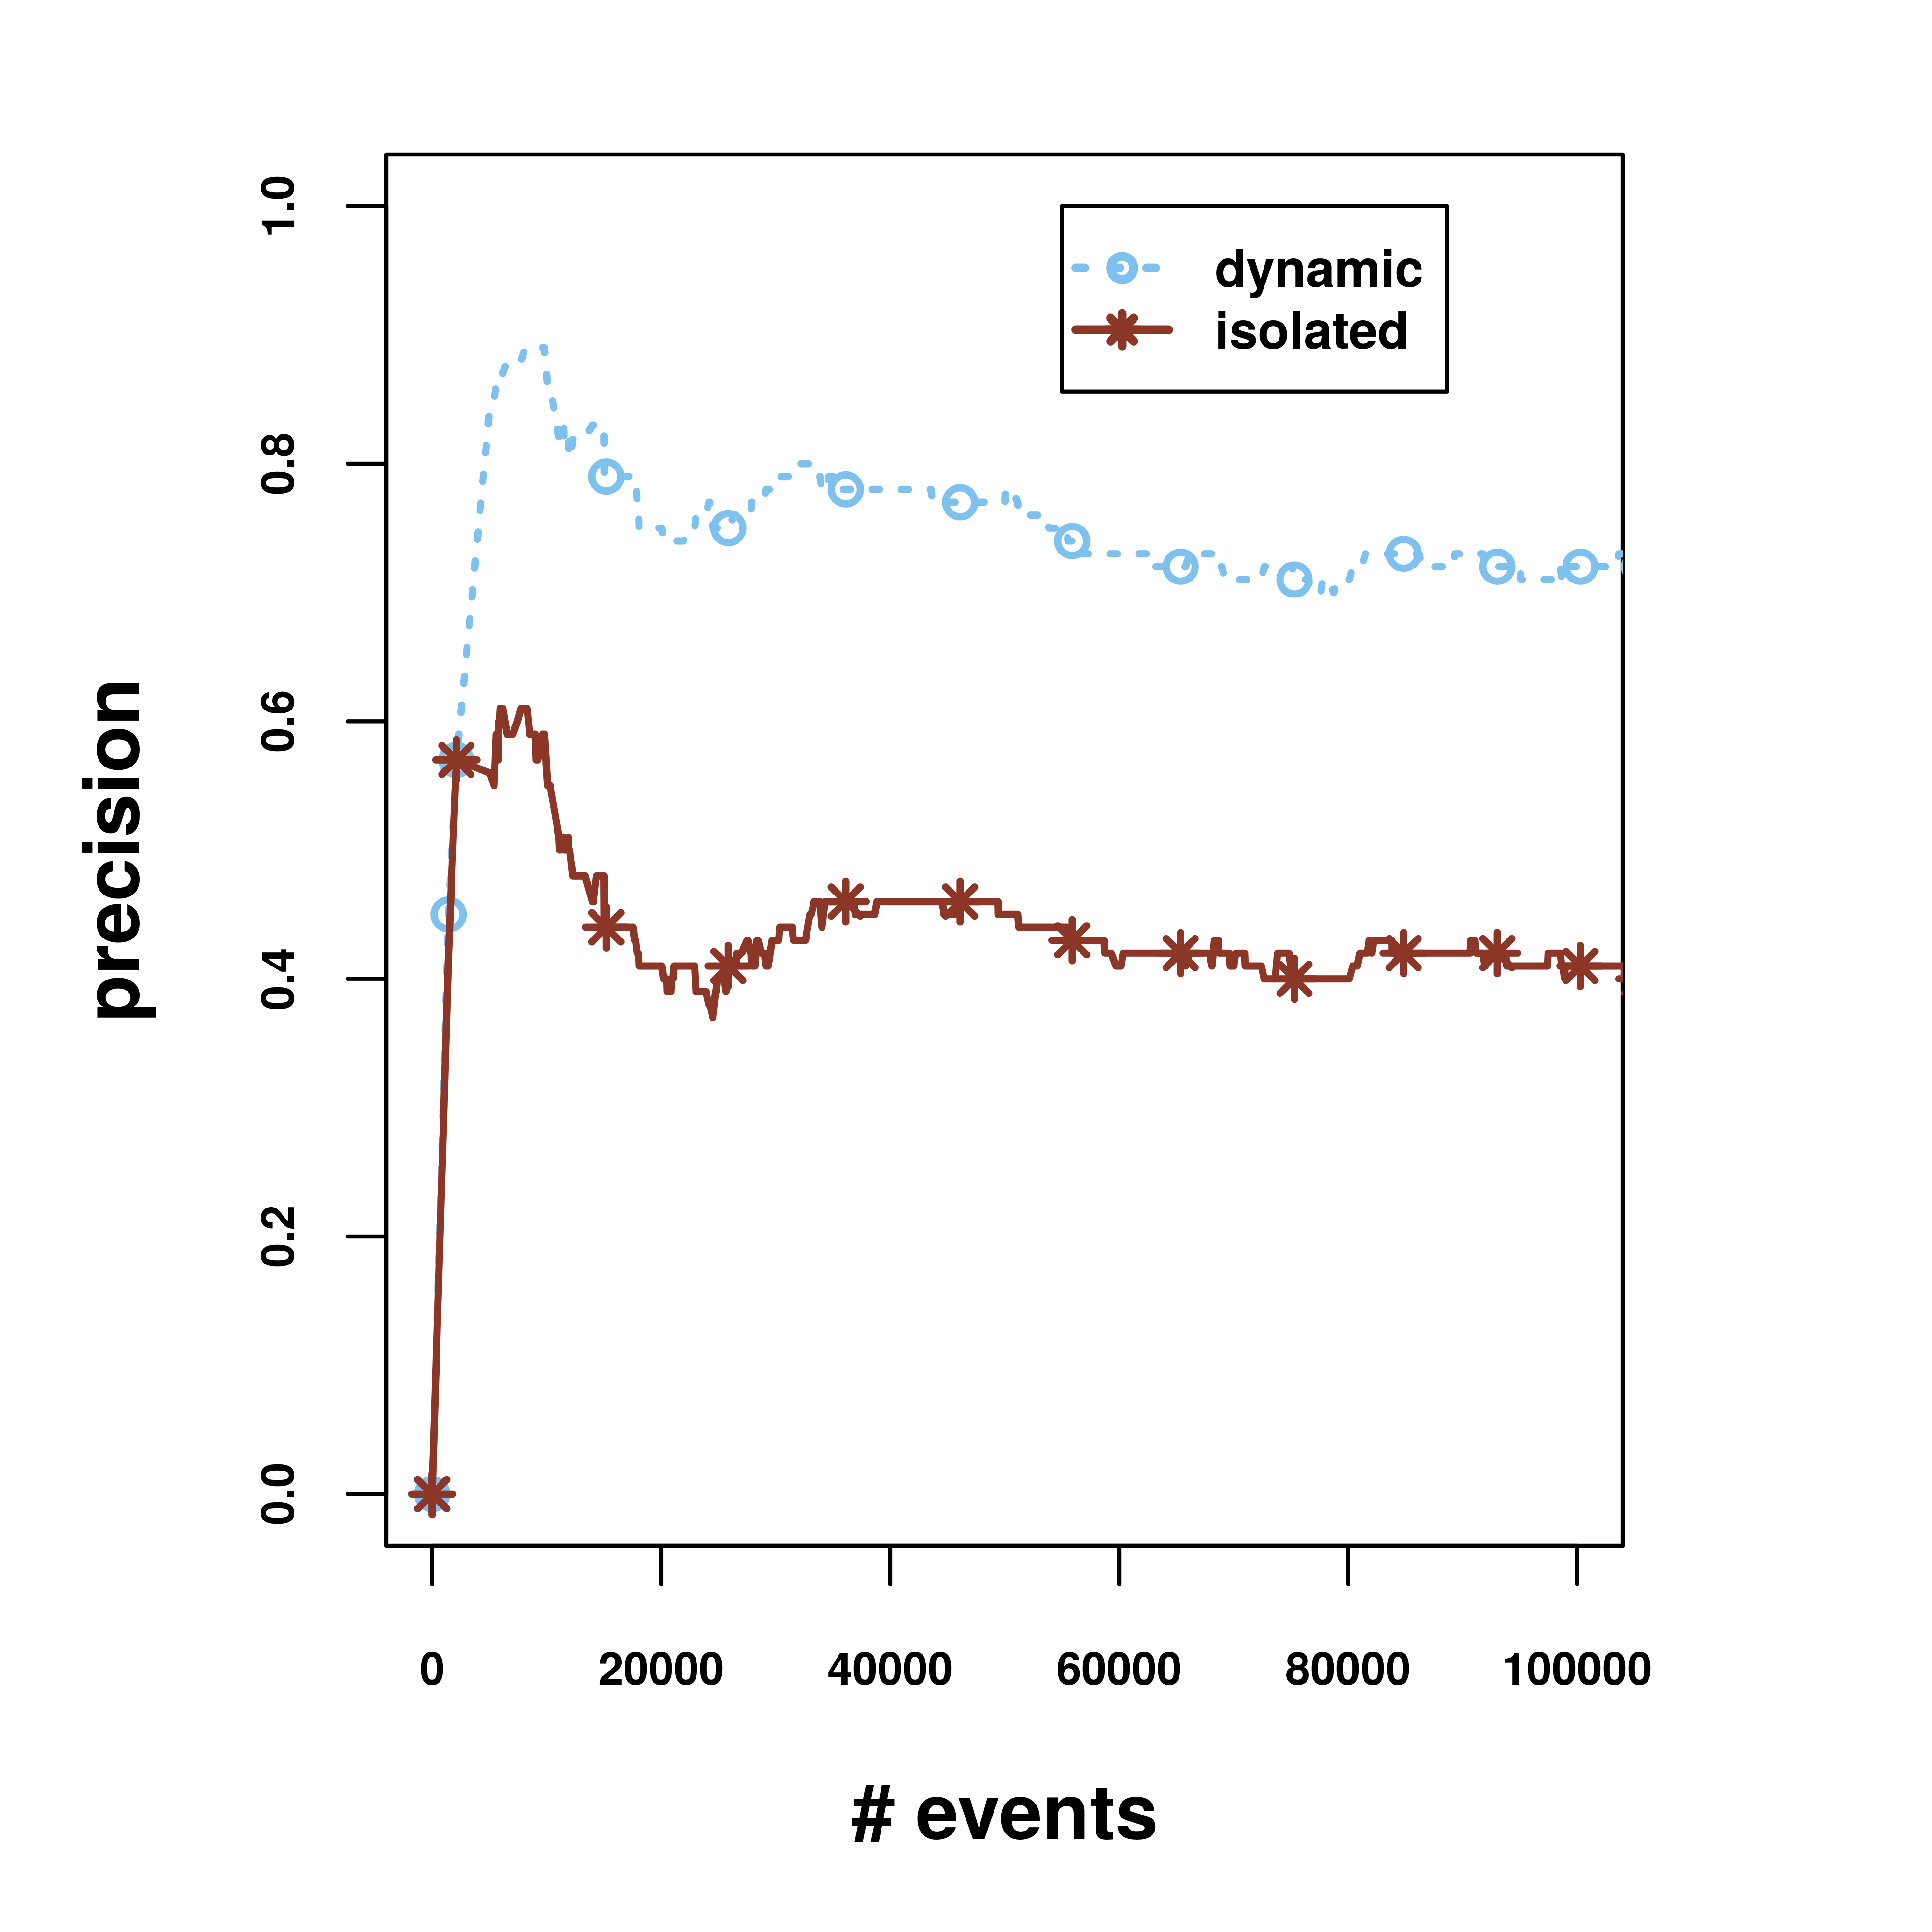
\includegraphics[width=\textwidth,keepaspectratio]{chapters/figures/synopses/new/precision_p2.png}
	
	\caption{Precision scores of $\mathcal{P}_2$  for vessels of \textit{pleasure craft} type.}
	\label{fig:precsions_p2}
\end{figure}

\section{Results on Synthetic Event Streams}
\label{sec:results_synthetic}
\FloatBarrier
We further extend the evaluation of our system by reporting the results of experiments for $\mathcal{P}=a ; d ; c$ over synthetically generated streams. We set the batch size to 20 ($b=20$), the variance threshold to .0001 ($\Delta=.0001$), the  \pmcmr prediction threshold to $50\%$ ($\theta_{p}=50\%$), and the maximum spread to 10 ($\theta_{s}=10$).
%


\begin{figure}[H]
	\centering
	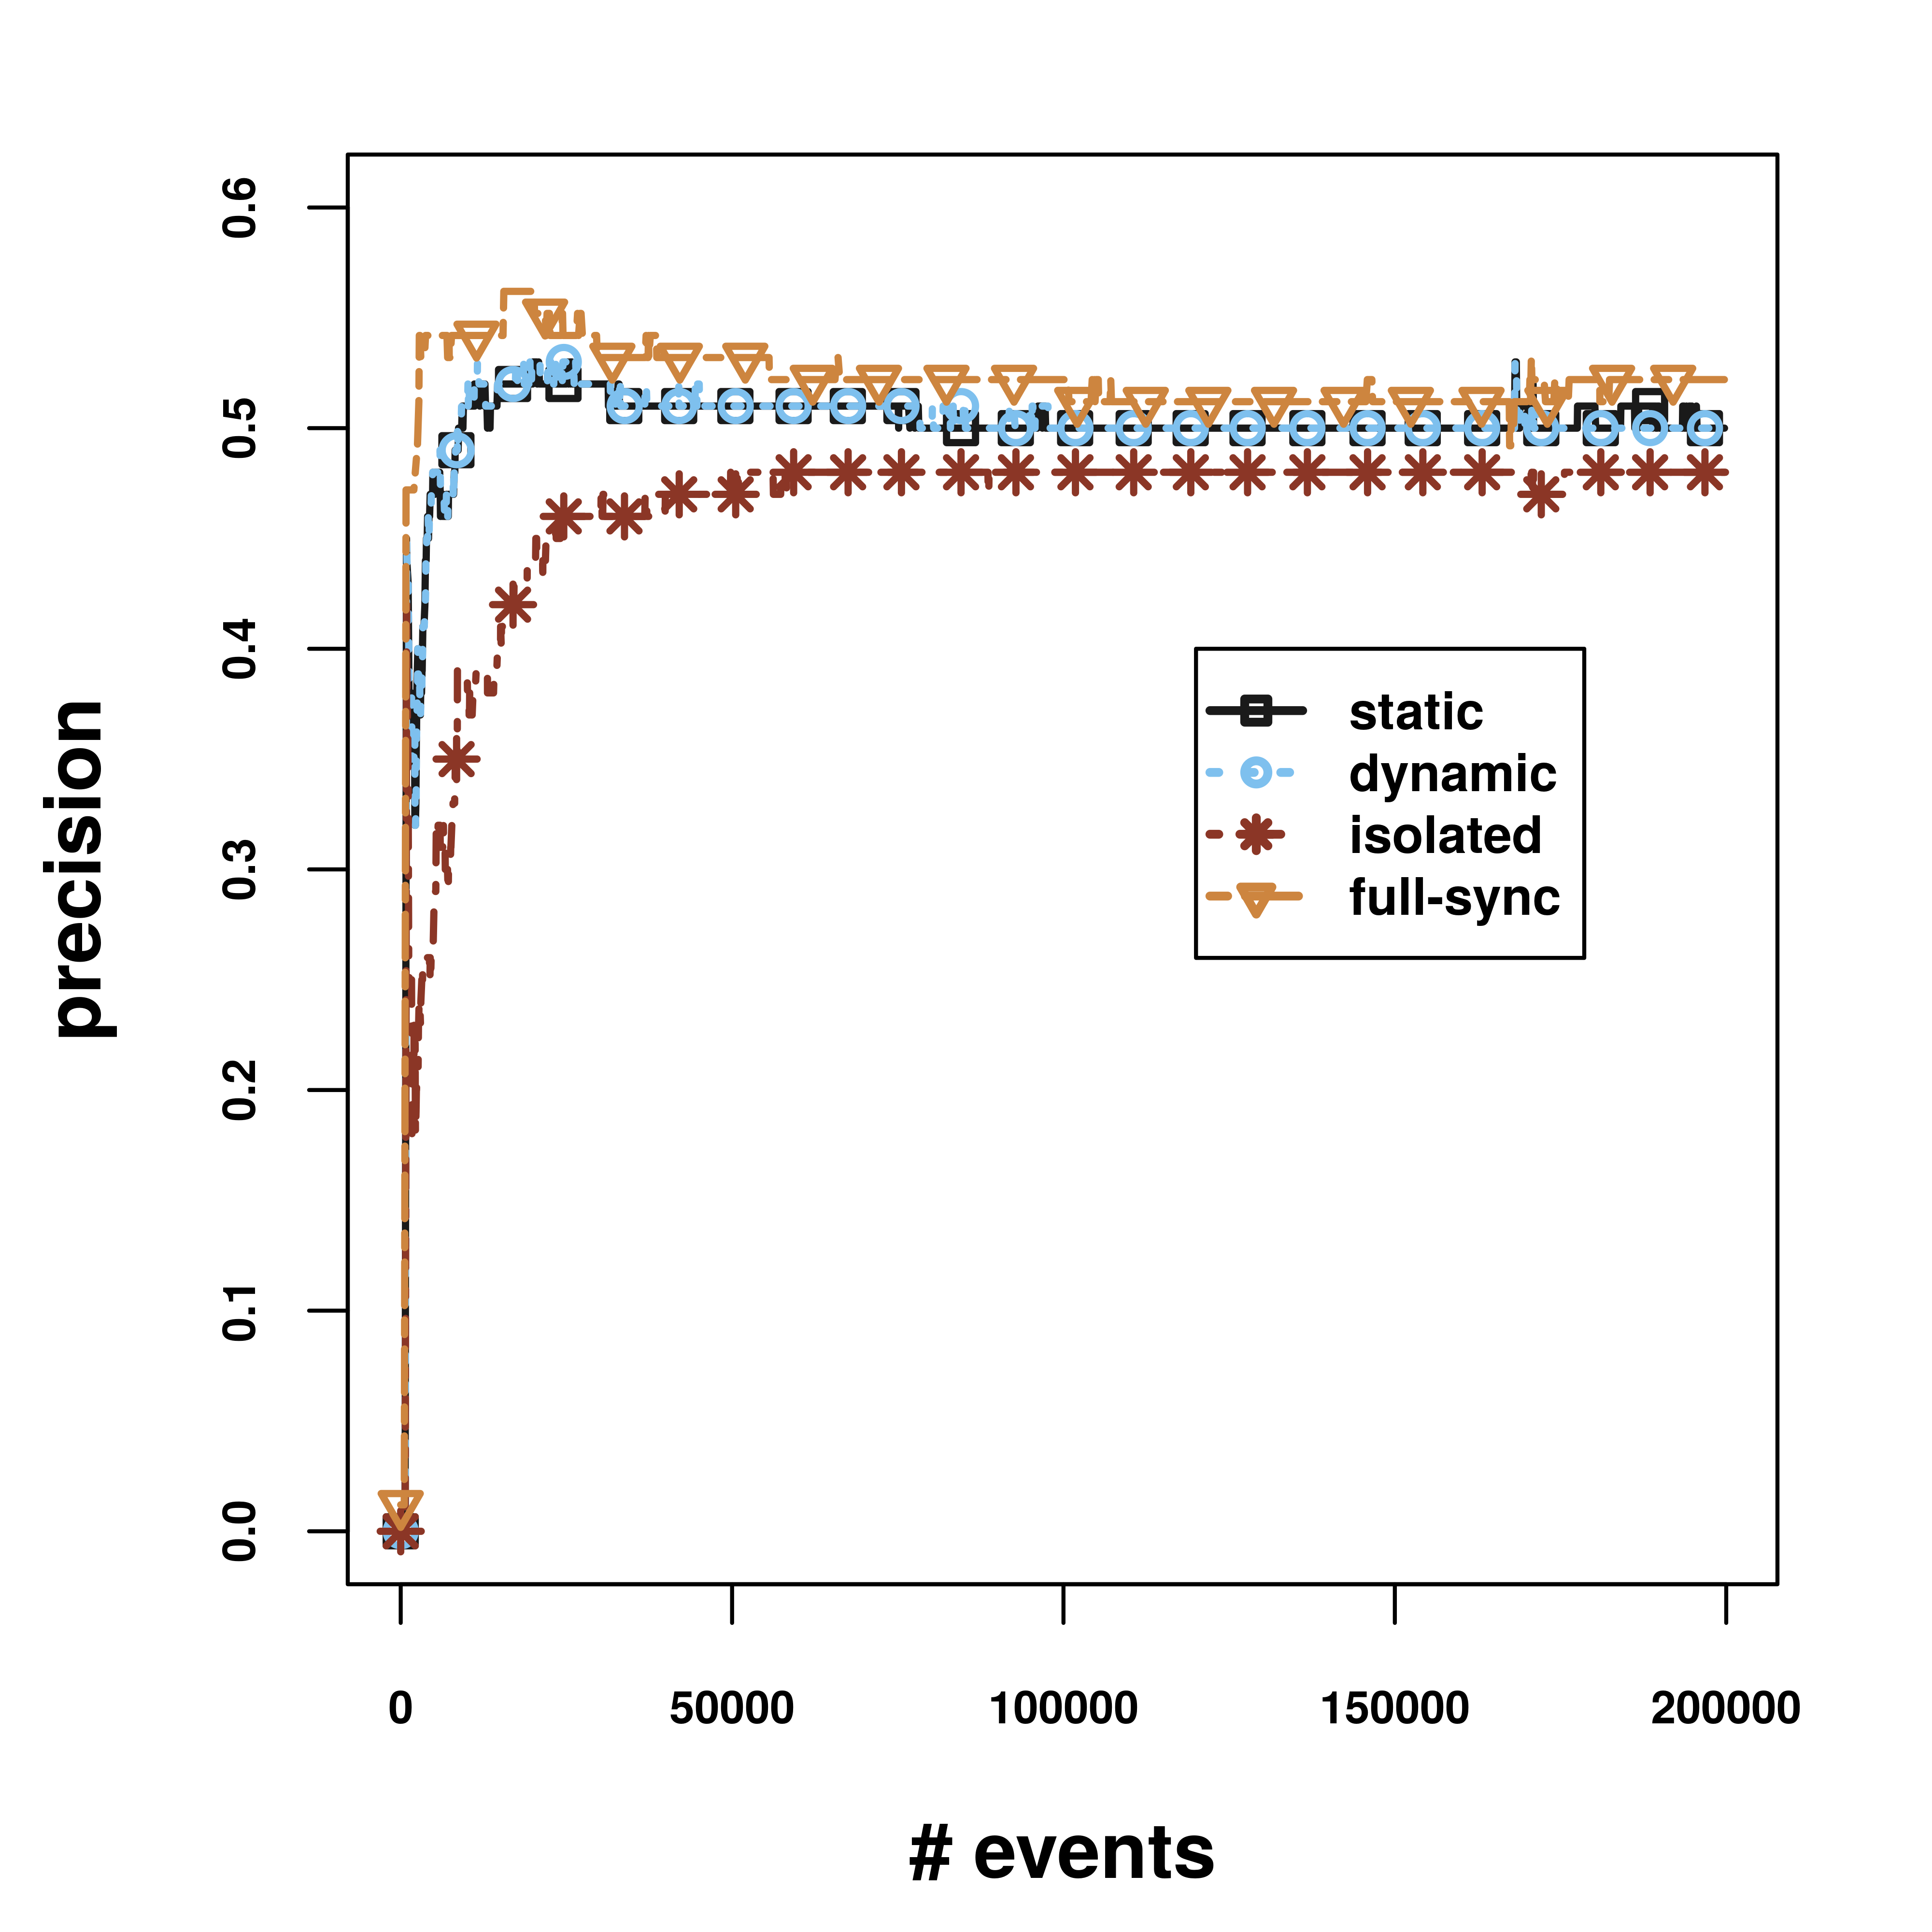
\includegraphics[width=\textwidth,height=.9\textwidth,keepaspectratio]{chapters/figures/synthetic/new/precision_synthetic.png}
	
	\caption{Precision scores with respect to the number of input events over time for $\mathcal{P}=a;d;c$.}
	\label{fig:precsion_synthetic}
\end{figure}

\par Figure~\ref{fig:precsion_synthetic} shows the average precision of the three modes of our system and the isolated approach. We can see that our proposed system in all its modes has higher precision scores than the isolated method. Also, it can be seen that the static and the dynamic approaches have similar performance while the more complex full synchronization mode has a slightly better performance. As expected, we also note that our method converges faster. The isolated models converge to the same accuracy but in much longer time.


\begin{figure}[H]
	\centering
	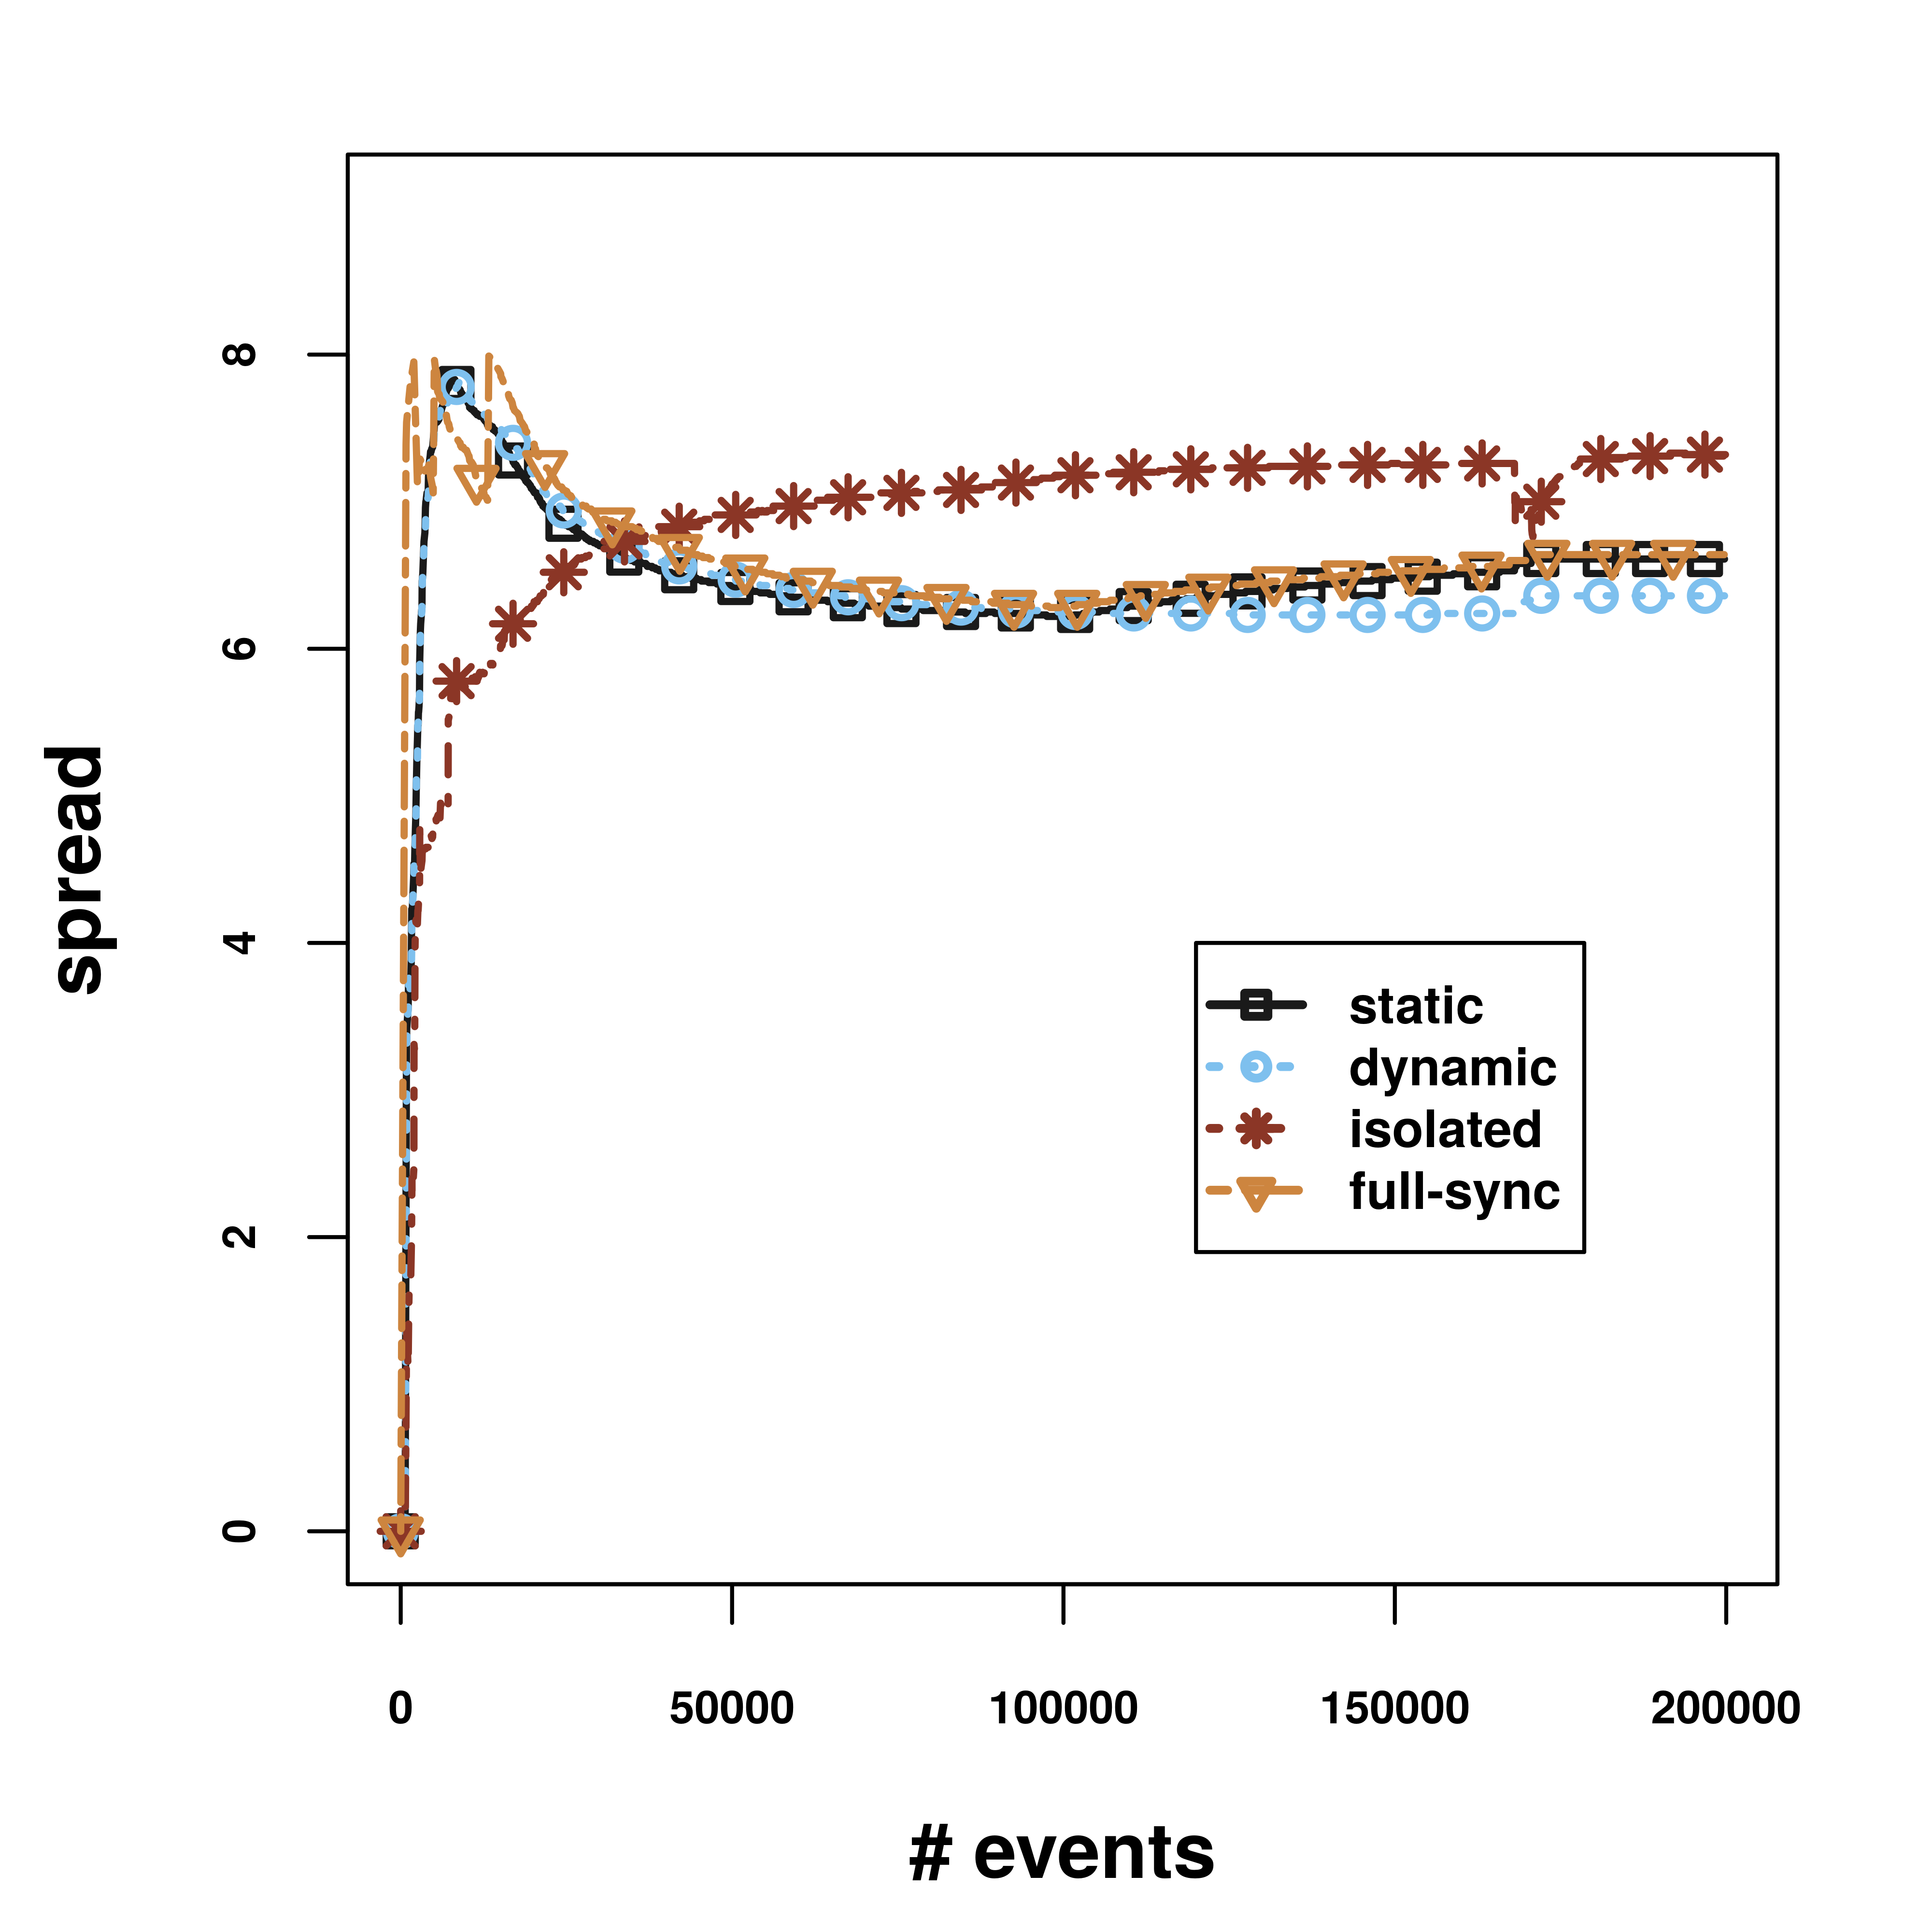
\includegraphics[width=\textwidth,height=.9\textwidth,keepaspectratio]{chapters/figures/synthetic/new/spread_synthetic.png}
	
	\caption{Average spread  with respect to the number of input events over time for $\mathcal{P}=a;d;c$.}
	\label{fig:spread_synthetic}
\end{figure}

\par On the other hand, Figure~\ref{fig:spread_synthetic} presents the average spread. As it can be seen, the average spread of the predictions in our approach (three modes) decreases after consuming more events. While the isolated approach has a higher spread that increases over time. 
\begin{figure}[H]
	\centering
	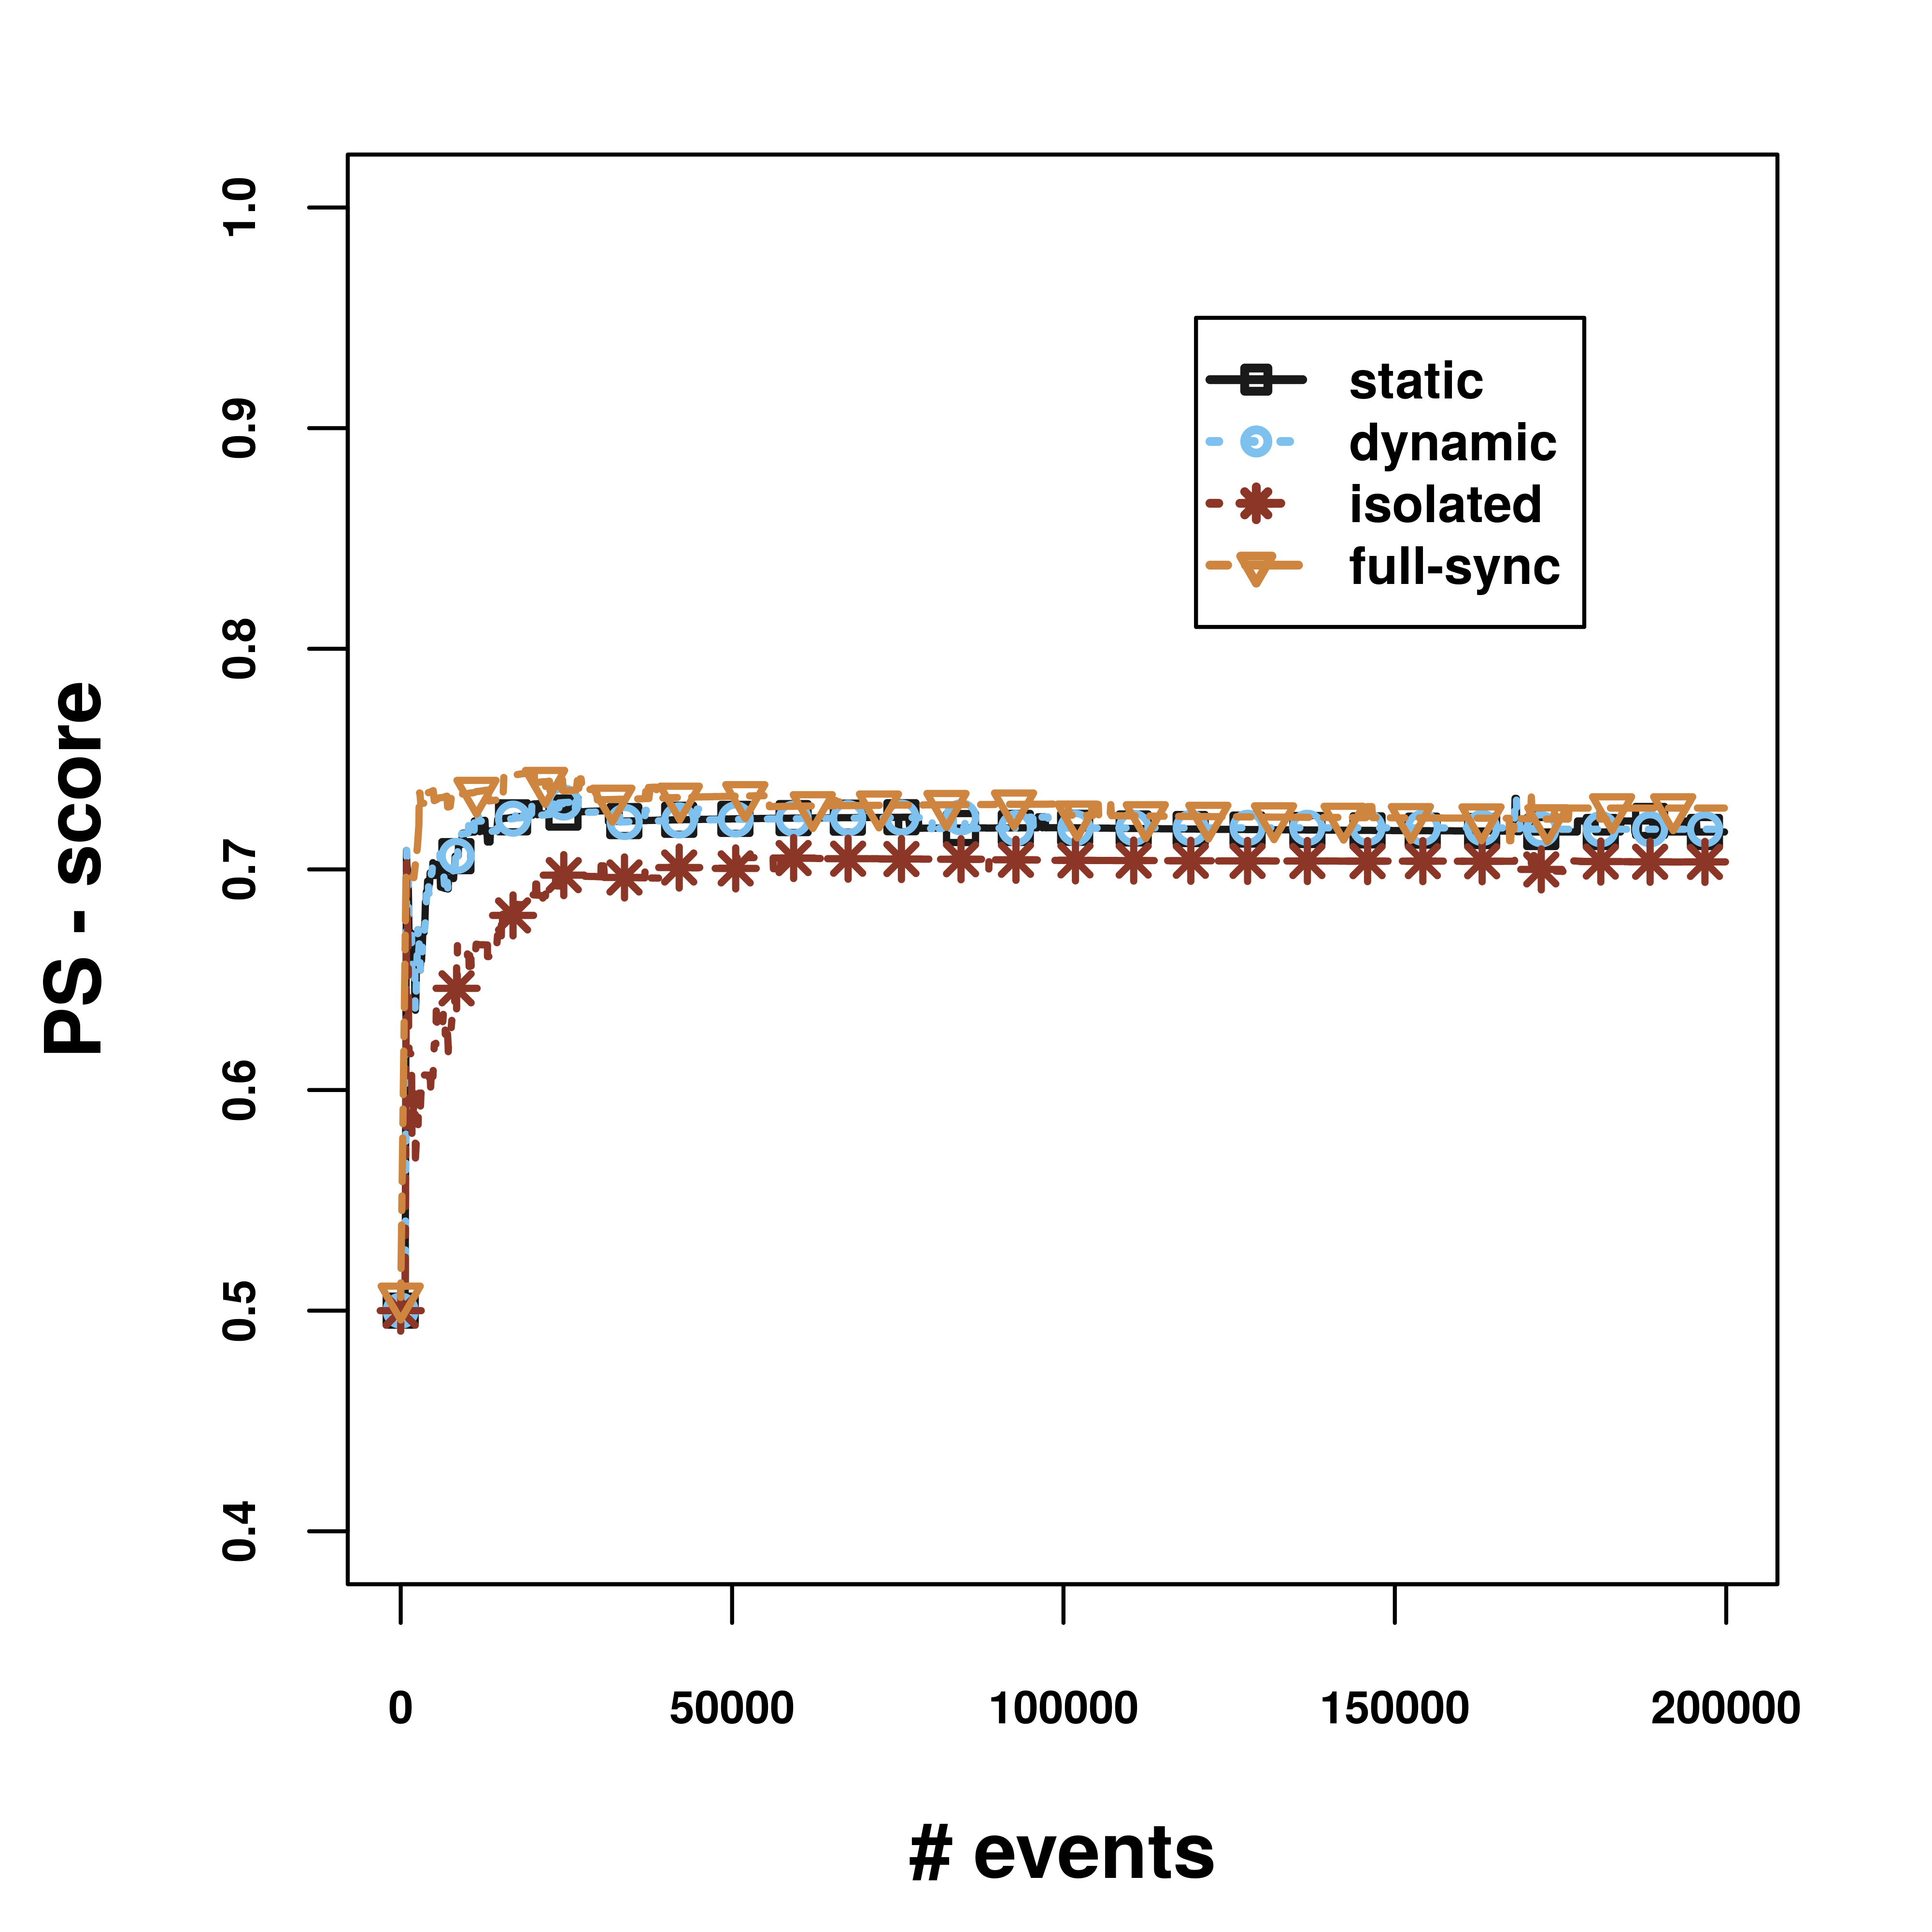
\includegraphics[width=\textwidth]{chapters/figures/synthetic/new/ps_score_synthetic.png}
	
	\caption{$\mathit{PS-score}$ for $\mathcal{P}=a;d;c$ with $\alpha = .5$.}
	\label{fig:ps_score_synth}
\end{figure}

\par Figure~\ref{fig:ps_score_synth} shows the $\mathit{PS}$-score of the different approaches. It can be seen that isolated converges slower than the three modes of our approach. Moreover, in Figure~\ref{fig:distance_synth}, it can be observed that the isolated has higher distance values compare to the different synchronization approaches. 

\begin{center}
	\centering
	\begin{figure}[H]
		
		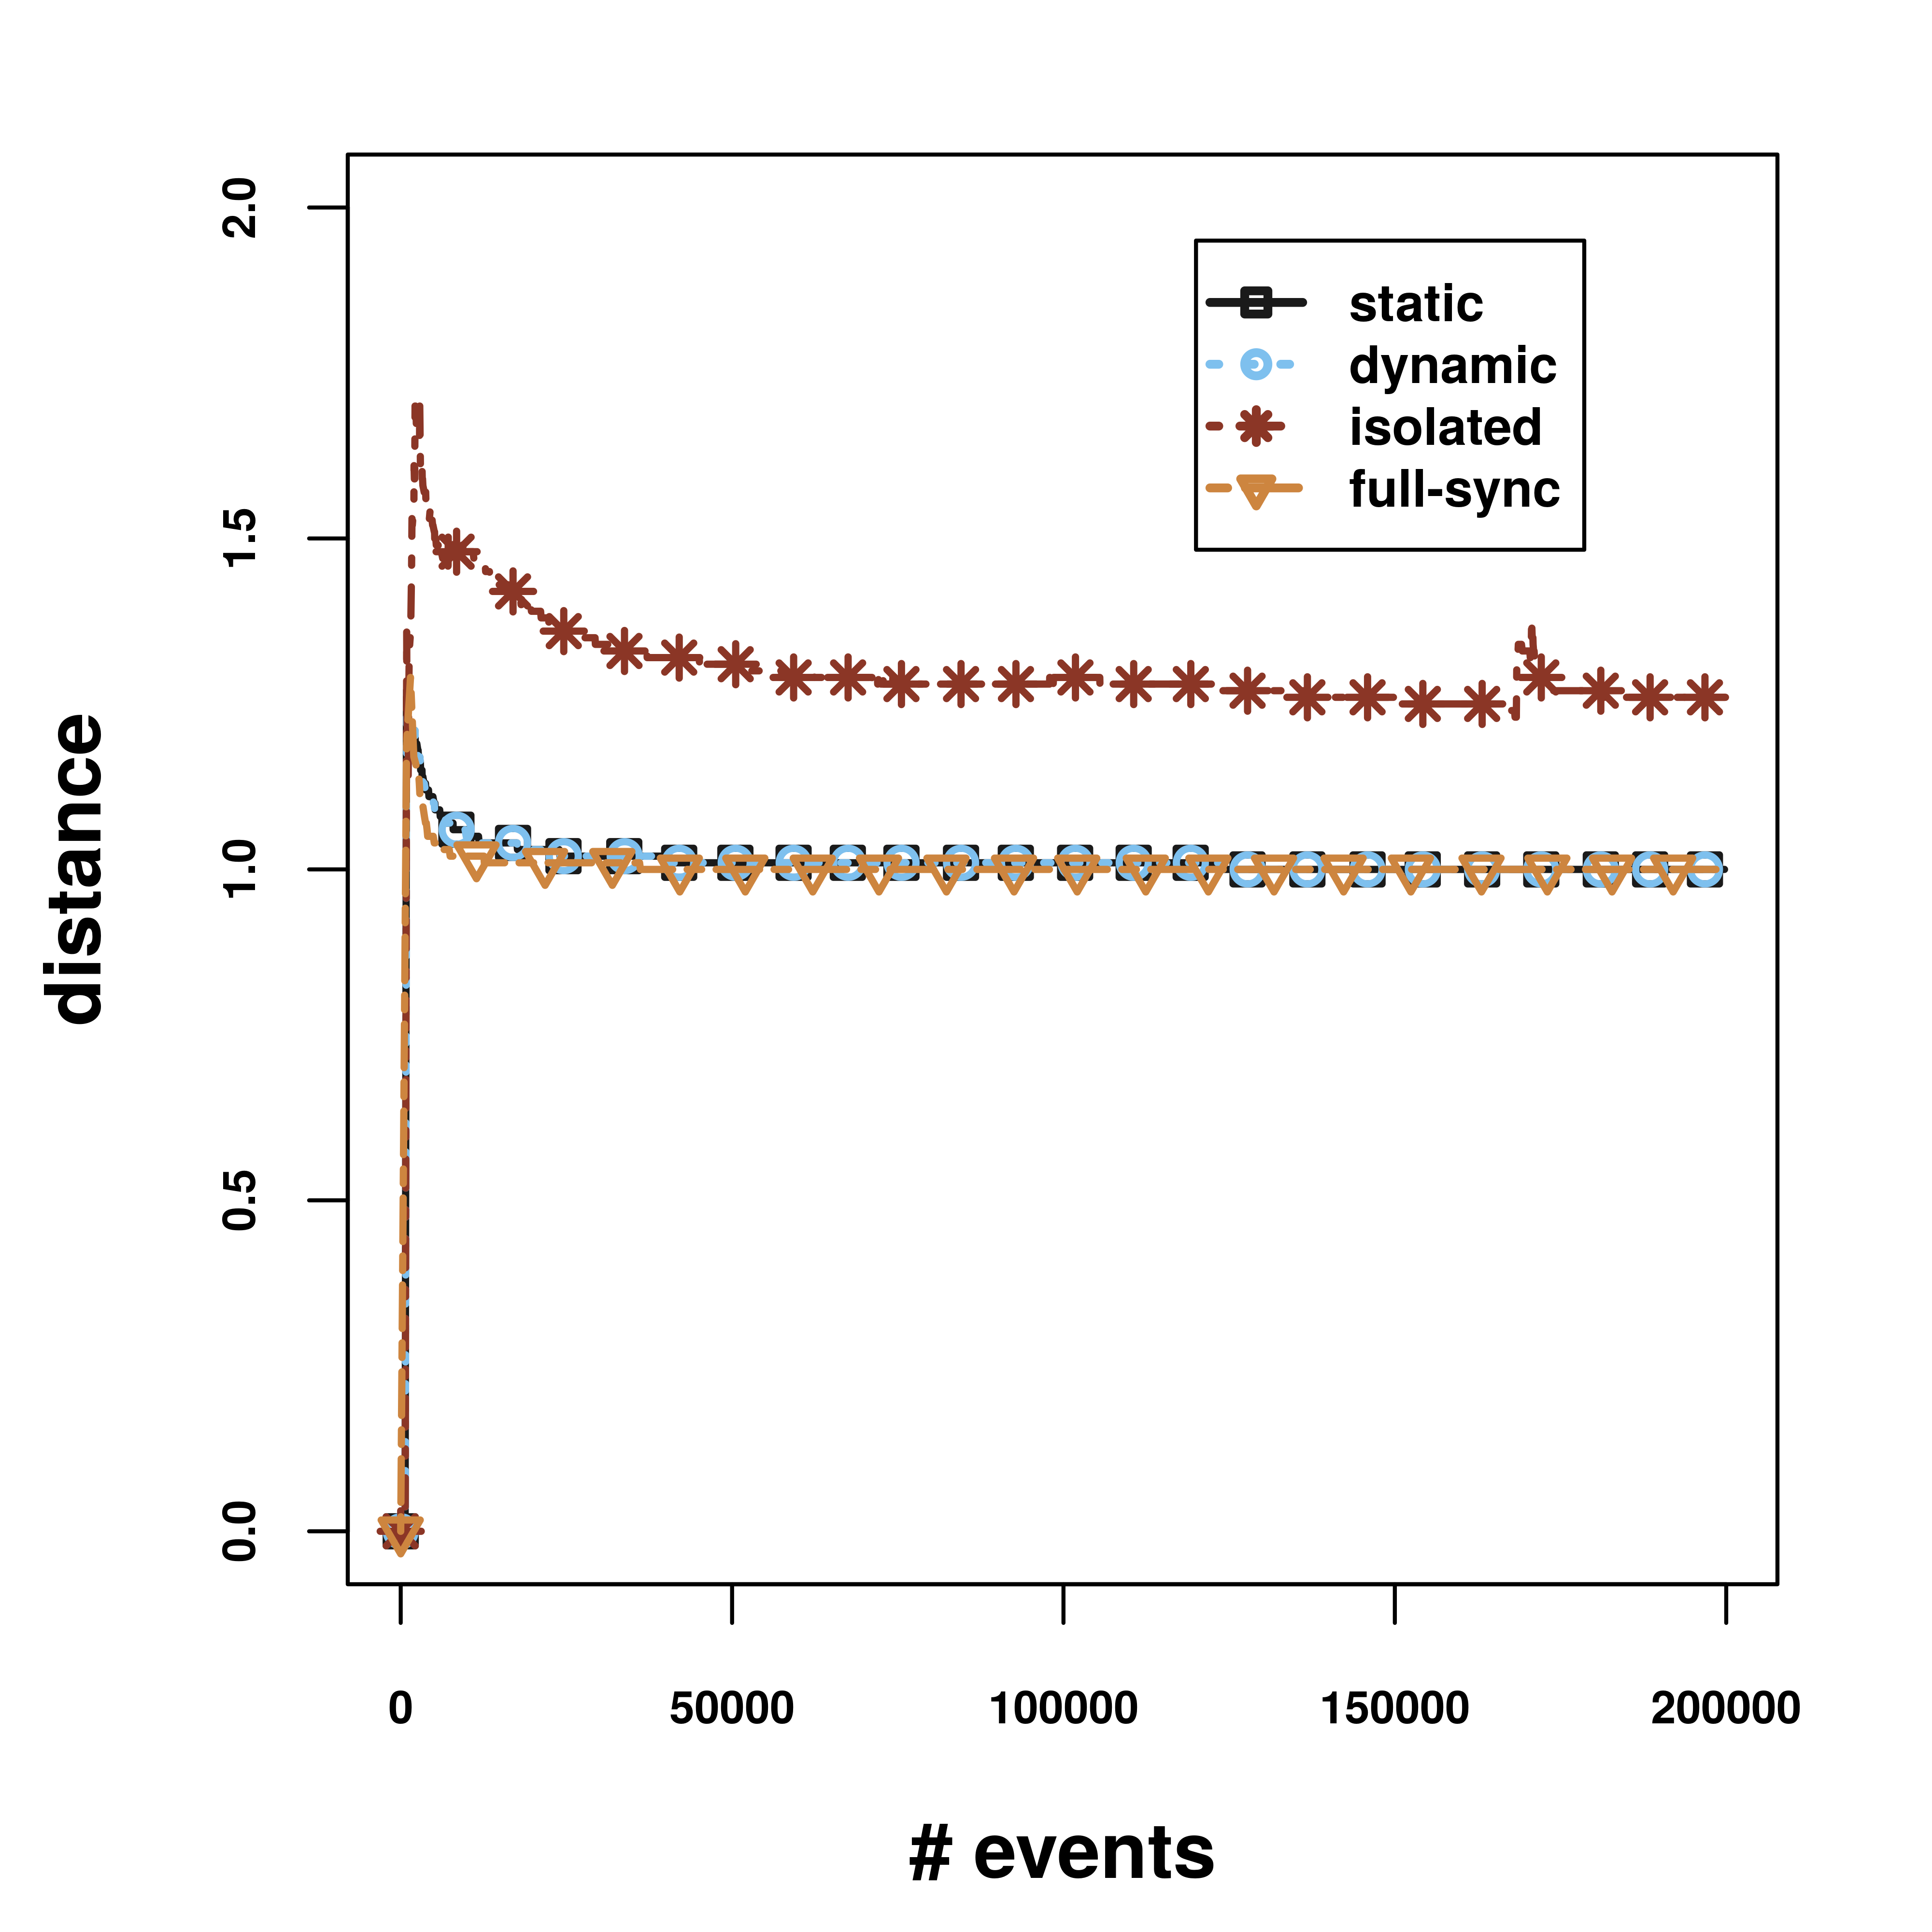
\includegraphics[width=\textwidth,keepaspectratio]{chapters/figures/synthetic/new/distance_synthetic.png}
		
		\caption{Distance measurements for $\mathcal{P}=a;d;c$.}
		\label{fig:distance_synth}
	\end{figure}
\end{center}

As discussed in Section ~\ref{sec:theoretical}, our proposed method improves the estimation of the transition probabilities of the underlying Markov chain for the \pmcmr models. Figure~\ref{fig:error_synthetic} shows the difference between the estimated transition probabilities and the reference probabilities of the Markov chain source ($\sum_{i,j} |\hat{p}_{i,j} - {p}_{i,j}|$), the results confirm the derived learning guarantee of our proposed approach that gives a better estimation of the transition probability matrix. It can be seen that the distributed modes have less estimation error and are faster in reaching the correct probabilities than the isolated approach. These results follow the probabilistic guarantee in Equation~\ref{eq:guarantee}.

\begin{figure}[H]
	\centering
	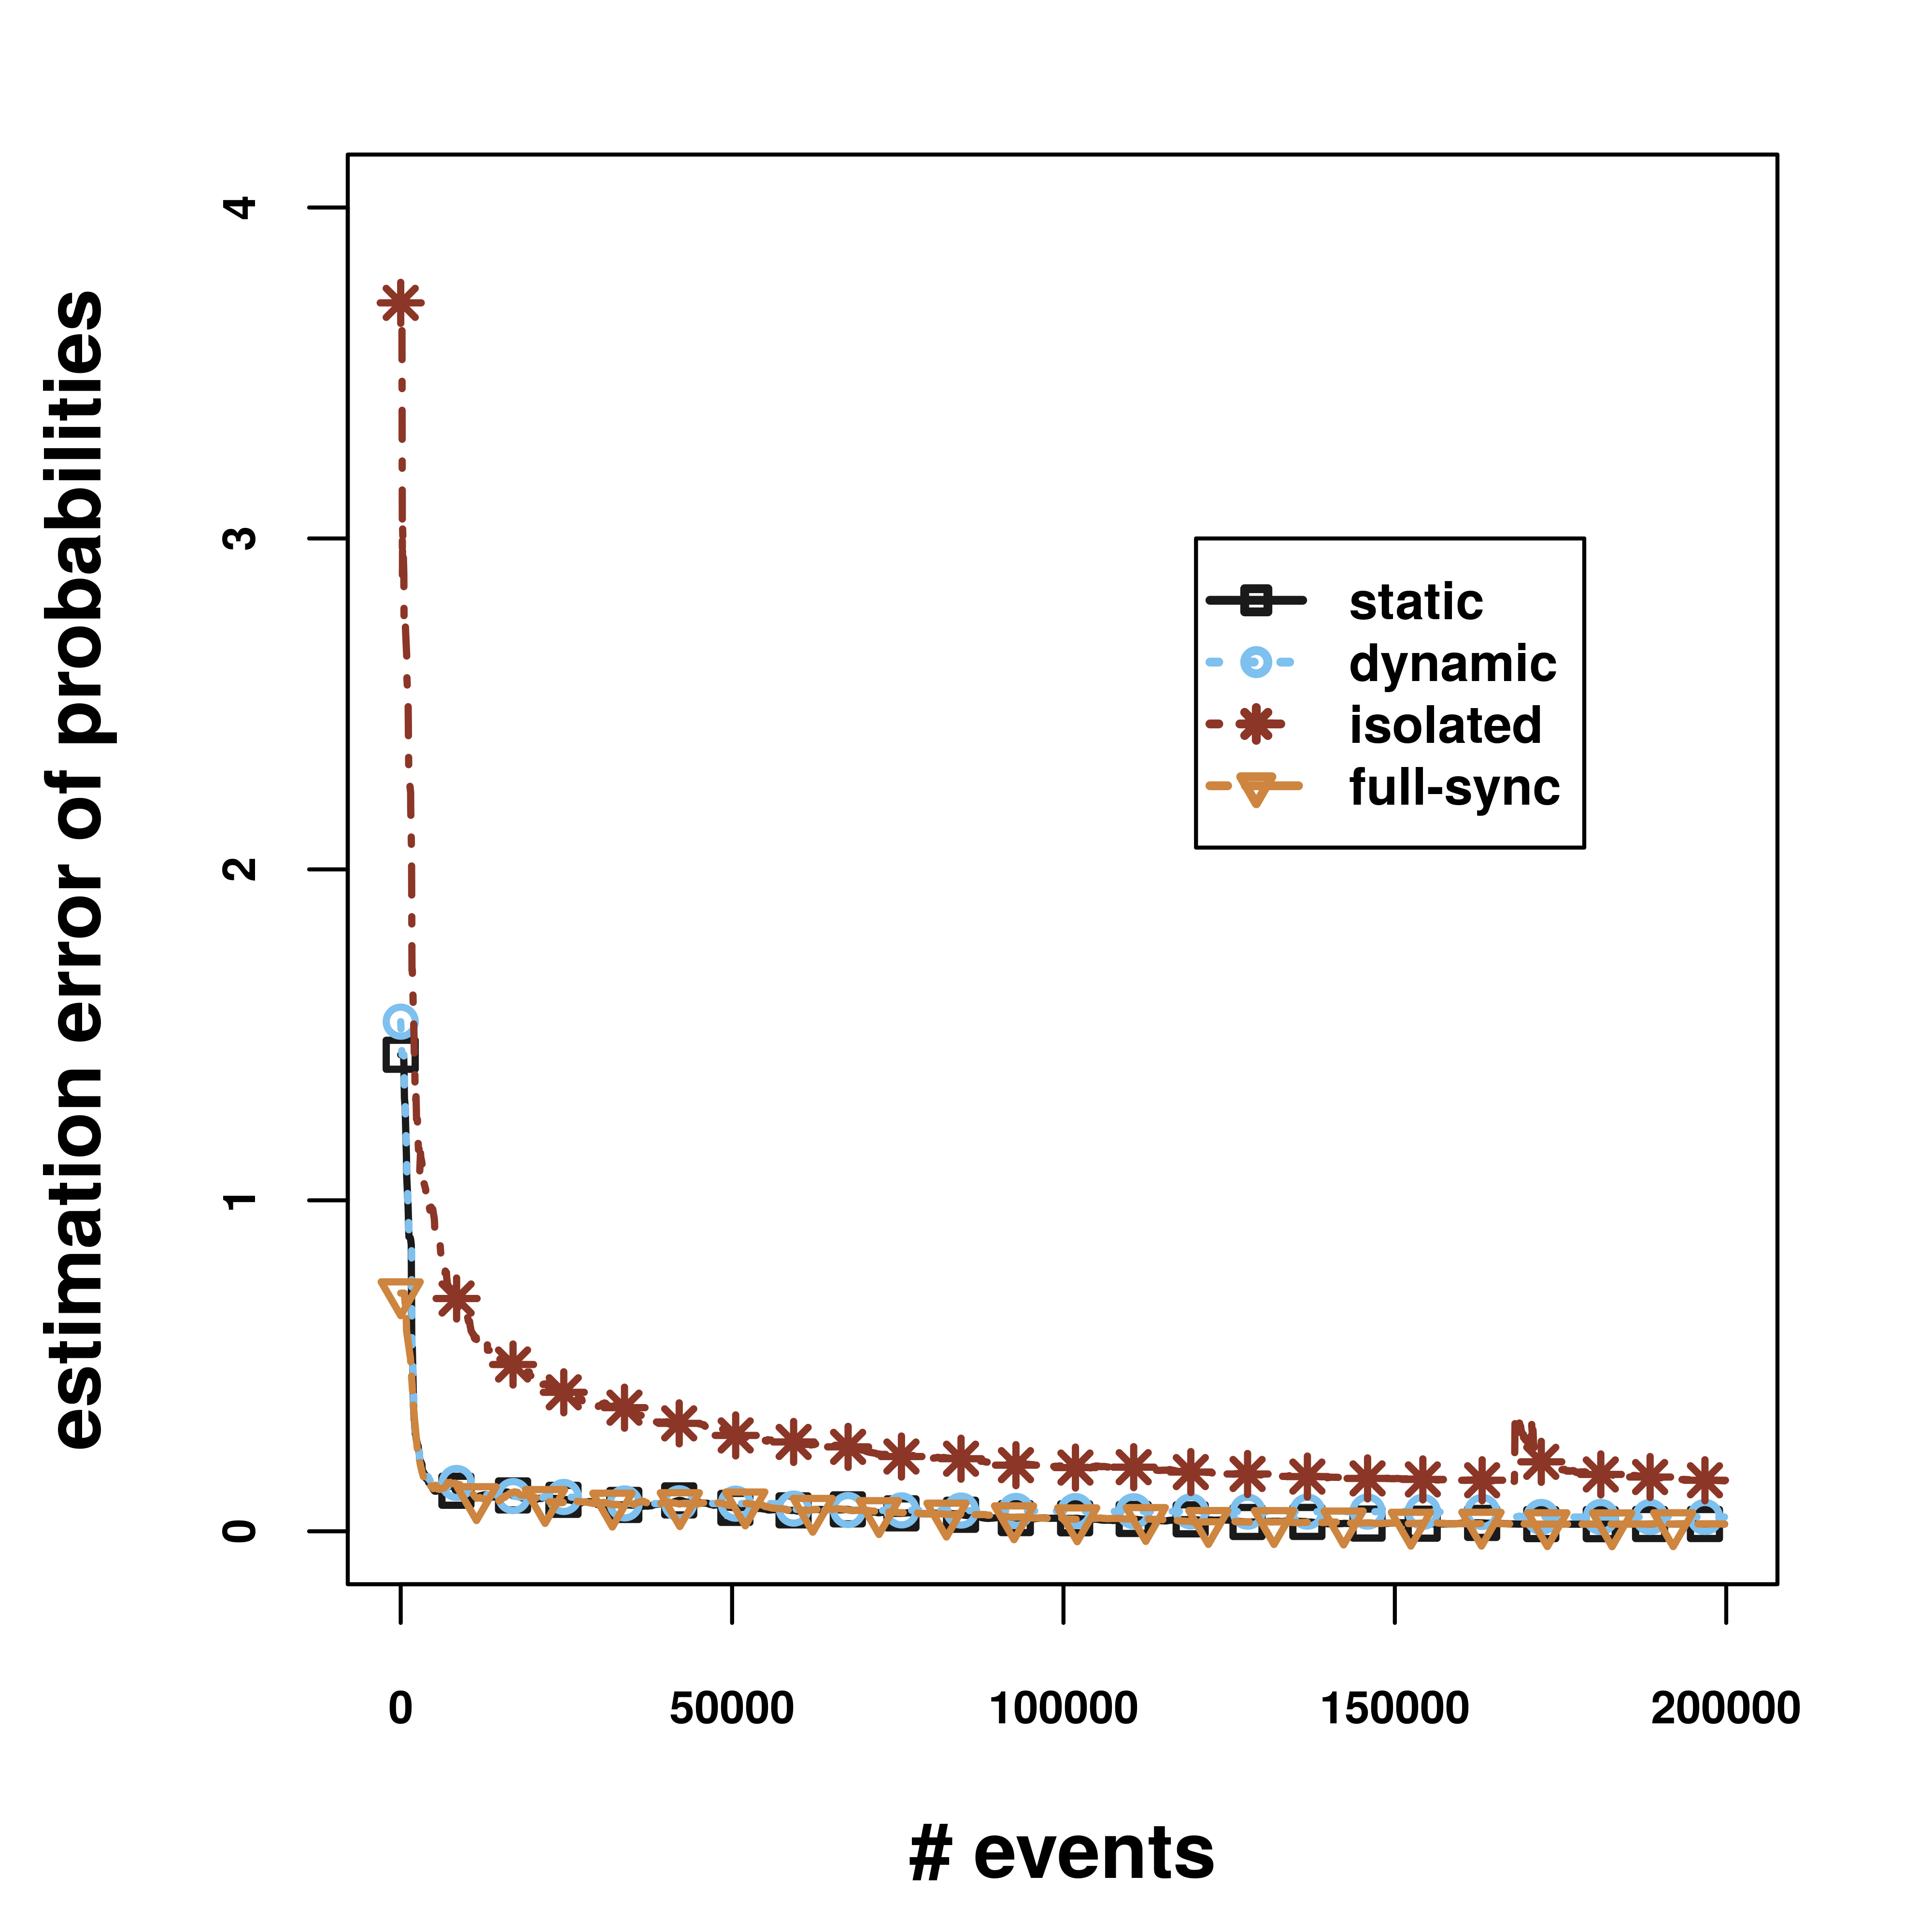
\includegraphics[width=\textwidth,keepaspectratio]{chapters/figures/synthetic/new/error_synthetic.png}
	
	\caption{The error  $\sum_{i,j} |\hat{p}_{i,j} - {p}_{i,j}|$) of estimating the transition probabilities  for $\mathcal{P}=a;d;c$.}
	\label{fig:error_synthetic}
\end{figure}




  


\section{Throughput Results}
\label{sec:throughput}

\begin{figure}[H]
	
	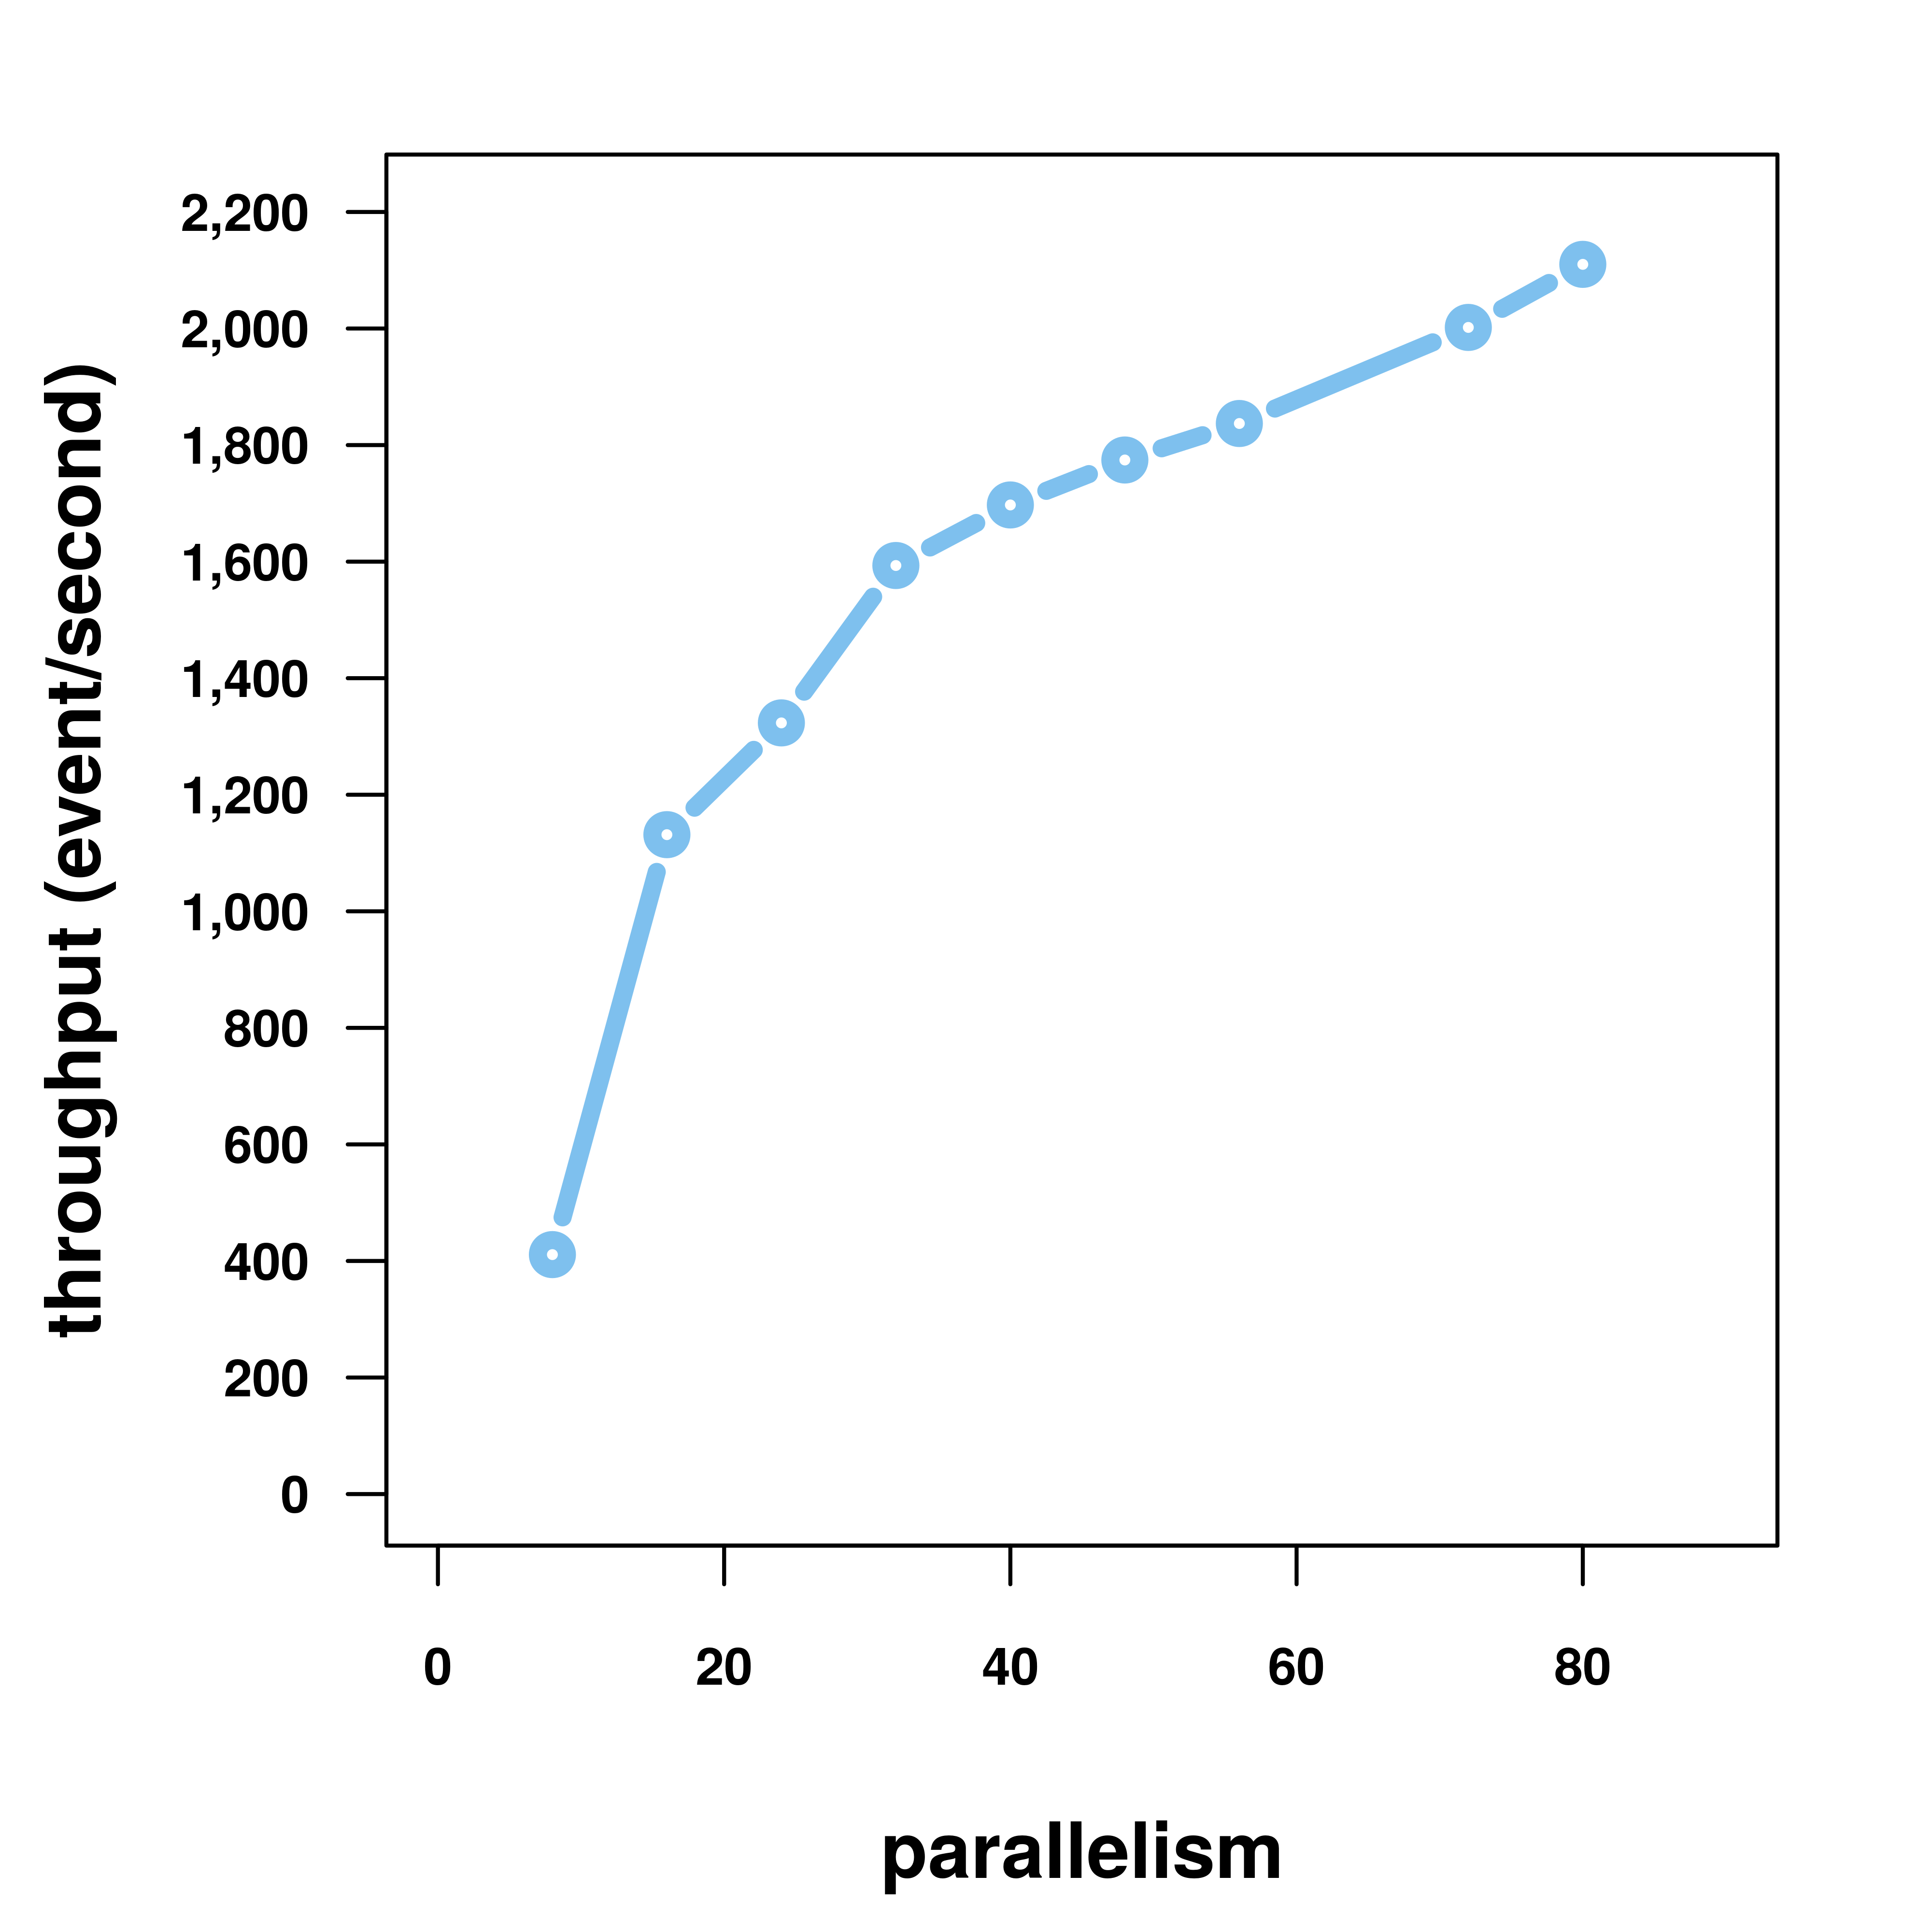
\includegraphics[width=\textwidth,keepaspectratio]{chapters/figures/throughput/temp.png}
	
	\caption{Throughput of the system on \ac{yarn} cluster in in terms of number of events processed per second with respect to the parallelism level over $\mathcal{P}_1$ with batch size $b=100$ and divergence threshold $\Delta=2$.}
	\label{fig:throughput}
\end{figure}


Figure~\ref{fig:throughput} reports the performance of the system  in terms of processing throughput on the YARN cluster using the first pattern $\mathcal{P}_1$. The dynamic synchronization scheme is performed. As we can observe, our system is capable of increasing the throughput by utilizing the distributed processing nodes based on the configured value for the Flink's parallelism level. 
\par It can also be seen that as we scale up by increasing the parallelism , the throughput grows by a factor of 5 ($5X$) from $\simeq\ 400\ $ events per second to $\simeq\ 2000\ $ events per second. However, notice that the system's throughput does not scale up linearly as the parallelism level increases. This can be explained by the fact that increasing the parallelism increases the network overhead to perform the models synchronization between the parallel predictors. Increasing number of the parallel predictors increases the number of the required synchronization phases.














%\par In Table ~\ref{tab:recall}, we present the mean of the recall scores for the both patterns in the all approaches It can be seen that the different approaches have a close recall scores, while the most frequent pattern ($\mathcal{P}_1$) has a lower recall than $\mathcal{P}_2$.
%
%\begin{table}[h]
%	\caption{Average recall for  $\mathcal{P}_1$ and $\mathcal{P}_2$.}
%	\label{tab:recall}
%	\begin{tabular}{lcc}
%		\toprule
%		Approach &Mean recall for $\mathcal{P}_1$ &Mean recall for $\mathcal{P}_2$\\
%		\midrule
%		isolated & 0.1707  &0.947 \\
%		static & 0.1754  &  0.960 \\
%		dynamic & 0.174  & 0.0.964 \\
%		full-sync & 0.1817  & 0.972 \\
%		\bottomrule
%	\end{tabular}
%\end{table}







 
